% This structure conforms to the mcgill university wide thesis guidelines:
% 
% https://www.mcgill.ca/gps/thesis/thesis-guidelines/preparation
% Some parts of it were taken from here, but mostly it is a "from scratch" template with minimal bload and fuzz: https://github.com/juliengs/mcgill-thesis-template
% Author: Maximilian Schiedermeier

\documentclass[12pt,oneside]{book}
\usepackage{graphicx}

% enable onehalfspaceing etc
\usepackage{setspace}

% Make chapter enumeration big and fat
\usepackage{fix-cm}
\usepackage{xcolor}
\usepackage[bf,rm,medium,compact]{titlesec}
\definecolor{gray75}{gray}{0.75}
\newcommand{\hsp}{\hspace{20pt}}
\titleformat{\chapter}[display]{\filleft\Huge\bfseries}{\fontsize{100}{100}\selectfont\textcolor{gray75}\thechapter}{1ex}{}[]%

% Enable non-ugly hyperlinks
\usepackage{blindtext}
\usepackage{epigraph}
\usepackage{multicol}

\usepackage{dsfont}
\usepackage{stmaryrd}
\usepackage{colortbl}
\usepackage{hyperref}

\usepackage{amsmath}
\DeclareMathOperator*{\argmax}{argmax}
\DeclareMathOperator*{\argmin}{argmin}
\usepackage{amssymb}

\usepackage[dvipsnames, table]{xcolor}
\usepackage{textcomp}

% Packages
\usepackage[pdf]{graphviz}
\usepackage{mathrsfs}

\newcommand*\circled[1]{\tikz[baseline=-0.1cm]{
  \node[shape=circle,draw,inner sep=0.48pt] (char) {\fontsize{7}{12}\textsf{#1}};}}

\DeclareMathAlphabet{\mathcal}{OMS}{cmsy}{m}{n}
\usepackage{cancel}
\newcommand\ccancel[2][red]{\renewcommand\CancelColor{\color{#1}}\cancel{#2}}
\newcommand{\nDownarrow}{\ensuremath{\text{ }\cancel{\Downarrow}\text{ }}}
\usepackage{centernot}

\usepackage{pgfplots, pgfplotstable}
\pgfplotsset{compat=1.7}
\usepgfplotslibrary{fillbetween}
\usetikzlibrary{patterns}
\pgfmathdeclarefunction{gauss}{2}{\pgfmathparse{1/(#2*sqrt(2*pi))*exp(-((x-#1)^2)/(2*#2^2))}}
\pgfmathdeclarefunction{nil}{1}{\pgfmathparse{0.001}}

\usepackage{arydshln}
\usepackage{adjustbox}
\usepackage{enumerate}
\usepackage{enumitem}
\usepackage{tikz-cd}
\usetikzlibrary{calc}
\usepackage{amsfonts}
%\usepackage{prooftrees}
\usepackage{bussproofs}
\renewcommand{\sectionautorefname}{\S}
\renewcommand{\subsectionautorefname}{\S}
\usepackage{float}

\usepackage{tikz-3dplot}
\usetikzlibrary{3d}
\usetikzlibrary{calligraphy}
\newif\ifshowcellnumber
\showcellnumbertrue

\usepackage{algorithm}
\usepackage[noend]{algpseudocode}
\usepackage{algorithmicx}
\usepackage{sourcecodepro}
\usepackage{tikz-qtree}
\usepackage{amsthm}
\usepackage{bm}
\usetikzlibrary{bayesnet}
\usetikzlibrary{arrows}
\usepackage{subcaption}
\usetikzlibrary{backgrounds}
\usetikzlibrary{tikzmark}
\usetikzlibrary{hobby}

\usepackage{mwe}

\newcommand{\E}{\mathbb{E}}
\newcommand{\Var}{\mathrm{Var}}
\newcommand{\Cov}{\mathrm{Cov}}

\newcommand{\CompOrder}{\mathcal{O}}
\def\graphspace{\mathbf{G}}
\def\Uniform{\mbox{\rm Uniform}}
\def\Gaussian{\mbox{\rm Gaussian}}
\def\Bernoulli{\mbox{\rm Bernoulli}}
\def\Dirichlet{\mbox{\rm Dirichlet}}

\usepackage{mathtools}% superior to amsmath
\usepackage{tikz}
% Packages
\usepackage{listings}
\DeclareRobustCommand{\hlred}[1]{{\sethlcolor{pink}\hl{#1}}}
\usepackage{fontspec}

\setmonofont[Scale=0.8]{JetBrainsMono}[
  Contextuals={Alternate},
  Path=./font/,
  Extension = .ttf,
  UprightFont=*-Regular,
  BoldFont=*-Bold,
  ItalicFont=*-Italic,
  BoldItalicFont=*-BoldItalic
]

\usepackage[skins,breakable,listings]{tcolorbox}

\lstdefinelanguage{python}{
  comment=[l]{//},
  commentstyle={\color{gray}\ttfamily},
  emph={delegate, filter, firstOrNull, forEach, it, lazy, mapNotNull, println, repeat, assert, with, head, tail, len, return@},
  numberstyle=\noncopyable,
  identifierstyle=\color{black},
  keywords={abstract, actual, as, as?, break, by, class, companion, continue, data, do, dynamic, else, enum, expect, false, final, for, fun, get, if, import, in, infix, interface, internal, is, null, object, open, operator, override, package, private, public, return, sealed, set, super, suspend, this, throw, true, try, catch, typealias, val, var, vararg, when, where, while, tailrec, reified, from, import, def, yield, lambda, as, in, return, else, pass},
  keywordstyle={\bfseries},
  morecomment=[s]{/*}{*/},
  morestring=[b]",
  morestring=[s]{"""*}{*"""},
  ndkeywords={@Deprecated, @JvmField, @JvmName, @JvmOverloads, @JvmStatic, @JvmSynthetic, Array, Byte, Double, Float, Boolean, Int, Integer, Iterable, Long, Runnable, Short, String, int},
  ndkeywordstyle={\bfseries},
  sensitive=true,
  stringstyle={\ttfamily},
  literate={`}{{\char0}}1,
  escapeinside={(*@}{@*)}
}

\lstnewenvironment{smallpy}
{\lstset{
  basicstyle=\ttfamily\lst@ifdisplaystyle\footnotesize\fi,
  language=python
}}
{}

\lstdefinelanguage{tidy}{
  comment=[l]{//},
  commentstyle={\color{gray}\ttfamily},
  emph={|, ->, ---},
  emphstyle={\color{red}},
  identifierstyle=\color{black},
  keywords={\|, ->, ---},
  otherkeywords={|,->},
  morekeywords={|,->},
  keywordstyle={\color{blue}\bfseries},
  morecomment=[s]{/*}{*/},
  morestring=[b]",
  morestring=[s]{"""*}{*"""},
  ndkeywords={@Deprecated, @JvmField, @JvmName, @JvmOverloads, @JvmStatic, @JvmSynthetic, Array, Byte, Double, Float, Int, Integer, Iterable, Long, Runnable, Short, String},
  ndkeywordstyle={\color{orange}\bfseries},
  sensitive=true,
  stringstyle={\color{green}\ttfamily},
  literate={`}{{\char0}}1
}

%%%%%%%%%%%%%%%%%%%%%%%%%%%%%%%%%%%%%%%%%%%
%
% Color boxes
%
%%%%%%%%%%%%%%%%%%%%%%%%%%%%%%%%%%%%%%%%%%%

\tcbset{
  enhanced jigsaw,
  breakable,
  listing only,
%  boxsep=-1pt,
%  top=-1pt,
  bottom=0.1cm,
  right=0.5cm,
  overlay first={
    \node[black!50] (S) at (frame.south) {\Large\ding{34}};
    \draw[dashed,black!50] (frame.south west) -- (S) -- (frame.south east);
  },
  overlay middle={
    \node[black!50] (S) at (frame.south) {\Large\ding{34}};
    \draw[dashed,black!50] (frame.south west) -- (S) -- (frame.south east);
    \node[black!50] (S) at (frame.north) {\Large\ding{34}};
    \draw[dashed,black!50] (frame.north west) -- (S) -- (frame.north east);
  },
  overlay last={
    \node[black!50] (S) at (frame.north) {\Large\ding{34}};
    \draw[dashed,black!50] (frame.north west) -- (S) -- (frame.north east);
  },
  before={\par\vspace{5pt}},
  after={\par\vspace{\parskip}\noindent}
}

\definecolor{slightgray}{rgb}{0.90, 0.90, 0.90}

\usepackage{soul}
\makeatletter
\def\SOUL@hlpreamble{%
  \setul{}{3.0ex}%
  \let\SOUL@stcolor\SOUL@hlcolor%
  \SOUL@stpreamble%
}
\makeatother

\newcommand{\inline}[1]{%
  \begingroup%
  \sethlcolor{slightgray}%
  \hl{\ttfamily\footnotesize #1}%
  \endgroup
}

\newcommand{\tinline}[1]{%
  \begingroup%
  \sethlcolor{slightgray}%
  \hl{\ttfamily\tiny #1}%
  \endgroup
}

\newtcblisting{halftidyinput}[1][]{%
  left skip=0.7cm,
  left=0.35cm,
  width=6cm,
%  left=-0.01cm,
  top=-0.1cm,
  bottom=-0.35cm,
  listing options={
    language=tidy,
    basicstyle=\ttfamily\small,
%numberstyle=\footnotesize,
    showstringspaces=false,
    tabsize=2,
    breaklines=true,
    numbers=none,
    inputencoding=utf8,
    escapeinside={(*@}{@*)},
    #1
  },
  underlay unbroken and first={%
    \path[draw=none] (interior.north west) rectangle node[white]{\includegraphics[width=4mm]{../figures/tidyparse_logo.png}} ([xshift=-10mm,yshift=-7mm]interior.north west);
  }
}

\newtcblisting{wholetidyinput}[1][]{%
  left skip=0.7cm,
  left=0.35cm,
  top=0.1cm,
  middle=0mm,
  boxsep=0mm,
  listing options={
    language=tidy,
    basicstyle=\ttfamily\small,
%numberstyle=\footnotesize,
    showstringspaces=false,
    tabsize=2,
    breaklines=true,
    numbers=none,
    inputencoding=utf8,
    escapeinside={(*@}{@*)},
    #1
  },
  underlay unbroken and first={%
    \path[draw=none] (interior.north west) rectangle node[white]{\includegraphics[width=4mm]{../figures/tidyparse_logo.png}} ([xshift=-10mm,yshift=-9mm]interior.north west);
  }
}

\definecolor{A}{RGB}{6,150,104}
\definecolor{B}{RGB}{196,74,137}
\definecolor{C}{RGB}{117,237,133}
\definecolor{D}{RGB}{246,46,243}
\definecolor{E}{RGB}{89,162,12}
\definecolor{F}{RGB}{113,12,158}
\definecolor{G}{RGB}{191,205,142}
\definecolor{H}{RGB}{51,58,158}
\definecolor{I}{RGB}{244,212,3}
\definecolor{J}{RGB}{37,36,249}
\definecolor{K}{RGB}{253,165,71}
\definecolor{L}{RGB}{27,81,29}
\colorlet{LA}{A!30}
\colorlet{LB}{B!30}
\colorlet{LC}{C!30}
\colorlet{LD}{D!30}
\colorlet{LE}{E!30}
\colorlet{LF}{F!30}
\colorlet{LG}{G!30}
\colorlet{LH}{H!30}
\colorlet{LI}{I!30}
\colorlet{LJ}{J!30}
\colorlet{LK}{K!30}
\colorlet{LL}{L!30}
\newcommand{\hiliA}[1]{%
  \colorbox{LA}{$#1$}}
\newcommand{\hiliB}[1]{%
  \colorbox{LB}{$#1$}}
\newcommand{\hiliC}[1]{%
  \colorbox{LC}{$#1$}}
\newcommand{\hiliD}[1]{%
  \colorbox{LD}{$#1$}}
\newcommand{\hiliE}[1]{%
  \colorbox{LE}{$#1$}}
\newcommand{\hiliF}[1]{%
  \colorbox{LF}{$#1$}}
\newcommand{\hiliG}[1]{%
  \colorbox{LG}{$#1$}}
\newcommand{\hiliH}[1]{%
  \colorbox{LH}{$#1$}}
\newcommand{\hiliI}[1]{%
  \colorbox{LI}{$#1$}}
\newcommand{\hiliJ}[1]{%
  \colorbox{LJ}{$#1$}}
\newcommand{\hiliK}[1]{%
  \colorbox{LK}{$#1$}}
\newcommand{\hiliL}[1]{%
  \colorbox{LL}{$#1$}}
\newcommand{\highlight}[1]{%
  \colorbox{lgray}{$#1$}}
\colorlet{lred}{red!30}
\colorlet{lorange}{orange!30}
\colorlet{lgreen}{green!30}
\colorlet{lgray}{black!15}
\colorlet{dgray}{black!75}
\DeclareRobustCommand{\hlred}[1]{{\sethlcolor{lred}\hl{#1}}}
\DeclareRobustCommand{\hlorange}[1]{{\sethlcolor{lorange}\hl{#1}}}
\DeclareRobustCommand{\hlgreen}[1]{{\sethlcolor{lgreen}\hl{#1}}}
\DeclareRobustCommand{\hlgray}[1]{{\sethlcolor{lgray}\hl{#1}}}
\DeclareRobustCommand{\caret}[1]{{\sethlcolor{dgray}\textcolor{white}{\hl{#1}}}}

\usepackage{url}
\usepackage{qtree}

\usepackage{filecontents}
\usepackage{pstricks-add}
\usepackage{emoji}
\usepackage{alltt}
\usepackage{nicematrix}
\usepackage{graphicx}
\usepackage{ulem}
\usepackage{upquote}
\tikzstyle{every picture}+=[remember picture]
\usepackage{menukeys}
\pgfplotstableread[col sep=comma,]{timings_loc.csv}\loctimings
\pgfplotstableread[col sep=comma,]{timings_unloc.csv}\unloctimings

\makeatletter
\DeclareRobustCommand{\cev}[1]{%
    {\mathpalette\do@cev{#1}}%
}
\newcommand{\do@cev}[2]{%
  \vbox{\offinterlineskip
  \sbox\z@{$\m@th#1 x$}%
  \ialign{##\cr
  \hidewidth\reflectbox{$\m@th#1\vec{}\mkern4mu$}\hidewidth\cr
  \noalign{\kern-\ht\z@}
    $\m@th#1#2$\cr
  }%
  }%
}
\makeatother

\makeatletter
\DeclareRobustCommand{\pder}[1]{%
  \@ifnextchar\bgroup{\@pder{#1}}{\@pder{}{#1}}}
\newcommand{\@pder}[2]{\frac{\partial#1}{\partial#2}}
\makeatother

\newcommand{\shup}{\shortuparrow}
\newcommand{\shri}{\shortrightarrow}
\newcommand{\shur}{\shup\hspace{-5pt}\shri}

\makeatletter
\def\squigglyred{\bgroup \markoverwith{\textcolor{red}{\lower3\p@\hbox{\sixly \char58}}}\ULon}
\makeatother

\makeatletter
\def\squigglyblu{\bgroup \markoverwith{\textcolor{blue}{\lower3\p@\hbox{\sixly \char58}}}\ULon}
\makeatother

\makeatletter
\def\squigglyora{\bgroup \markoverwith{\textcolor{orange}{\lower3\p@\hbox{\sixly \char58}}}\ULon}
\makeatother

\newcommand{\err}[1]{\smash{\squigglyred{#1}{}}}
\newcommand{\erb}[1]{\smash{\squigglyblu{#1}{}}}
\newcommand{\ero}[1]{\smash{\squigglyora{#1}{}}}
\newcommand{\stirlingii}{\genfrac{\{}{\}}{0pt}{}}

%======== Arrows =========
\newcommand{\knightarrow}{
  \tikz{
    \fill (0pt,0pt) circle [radius = 1pt];
    \fill (0pt,6pt) circle [radius = 1pt];
    \fill (6pt,0pt) circle [radius = 1pt];
    \fill (6pt,6pt) circle [radius = 1pt];
    \fill (12pt,0pt) circle [radius = 1pt];
    \fill (12pt,6pt) circle [radius = 1pt];
    \fill (6pt,0pt) circle [radius = 1pt];
    \fill (12pt,0pt) circle [radius = 1pt];
    \draw [-to] (0pt,0pt) -- (12pt,6pt);
  }
}

\newcommand{\kingarrow}{
  \tikz{
    \fill (0pt,0pt) circle [radius = 1pt];
    \fill (6pt,0pt) circle [radius = 1pt];
    \fill (0pt,6pt) circle [radius = 1pt];
    \fill (6pt,6pt) circle [radius = 1pt];
    \draw [-to] (0pt,0pt) -- (6pt,6pt);
    \draw [-to] (0pt,0pt) -- (0pt,6pt);
    \draw [-to] (0pt,0pt) -- (6pt,0pt);
  }
}

\newcommand{\duparrow}{
  \tikz{
    \fill[white] (0pt,0pt) circle [radius = 1pt];
    \fill (6pt,0pt) circle [radius = 1pt];
    \fill (0pt,6pt) circle [radius = 1pt];
    \fill[white] (6pt,6pt) circle [radius = 1pt];
    \draw [-to] (6pt,0pt) -- (0pt,6pt);
  }
}

\newcommand{\drightarrow}{
  \tikz{
    \fill (0pt,0pt) circle [radius = 1pt];
    \fill (6pt,0pt) circle [radius = 1pt];
    \draw [-to] (0pt,0pt) -- (6pt,0pt);
  }
}

\newcommand{\ddiagarrow}{
  \tikz{
    \fill (0pt,0pt) circle [radius = 1pt];
    \fill (6pt,0pt) circle [radius = 1pt];
    \fill (0pt,6pt) circle [radius = 1pt];
    \fill (6pt,6pt) circle [radius = 1pt];
    \draw [-to] (0pt,0pt) -- (6pt,6pt);
  }
}

\newcommand{\knightkingarrow}{
  \tikz{
    \fill (0pt,0pt) circle [radius = 1pt];
    \fill (0pt,6pt) circle [radius = 1pt];
    \fill (6pt,0pt) circle [radius = 1pt];
    \fill (6pt,6pt) circle [radius = 1pt];
    \fill (12pt,0pt) circle [radius = 1pt];
    \fill (12pt,6pt) circle [radius = 1pt];
    \draw [-to] (0pt,0pt) -- (6pt,6pt);
    \draw [-to] (0pt,0pt) -- (0pt,6pt);
    \draw [-to] (0pt,0pt) -- (6pt,0pt);
    \draw [-to] (0pt,0pt) -- (12pt,6pt);
  }
}

%======== Arrows =========

\usetikzlibrary{decorations.pathreplacing,automata,calc,positioning,matrix,chains,fit,decorations.pathmorphing}

\usepackage{wrapfig}

\newcommand{\mkTrellis}[1]{
  \begin{tikzpicture}
  \def\dx{20pt}
  \def\dy{30pt}
  \newcounter{i}
  \stepcounter{i}
  \node[circle, draw, fill=black!30] (\arabic{i}) at (0,0){};
  \foreach [count=\i] \x in {2,...,#1}{
    \pgfmathsetmacro{\lox}{\x-1}%
    \pgfmathsetmacro{\loxt}{\x-3}%
    \foreach [count=\j] \xx in {-\lox,-\loxt,...,\lox}{
      \pgfmathsetmacro{\jj}{\j-1}%
      \stepcounter{i}
      \pgfmathsetmacro{\kk}{\xx-2}%
      \pgfmathsetmacro{\lbl}{\lox!/(\jj!*(\lox-\jj)!)}
      \ifnum\x<\kk
      \pgfmath\node[circle, draw]  (\arabic{i}) at (\xx*\dx, -\lox*\dy) {};
      \else
        \pgfmath\node[circle, draw, fill=black!30]  (\arabic{i}) at (\xx*\dx, -\lox*\dy) {};
      \fi
    }
  }
  \newcounter{z}
  \newcounter{xn}
  \newcounter{xnn}
  \pgfmathsetmacro{\maxx}{#1 - 1}
  \foreach \x in {1,...,\maxx}{
    \foreach \xx in {1,...,\x}{
      \stepcounter{z}
      \setcounter{xn}{\arabic{z}}
      \addtocounter{xn}{\x}
      \setcounter{xnn}{\arabic{xn}}
      \stepcounter{xnn}
      \draw [<-] (\arabic{z}) -- (\arabic{xn});
      \draw [<-] (\arabic{z}) -- (\arabic{xnn});
    }
  }
  \end{tikzpicture}
}

\newcommand{\dx}{20pt}
\newcommand{\dy}{30pt}
\newcounter{i}
\newcounter{z}
\newcounter{xn}
\newcounter{xnn}
\newcommand{\mkTrellisAppend}[1]{
  \begin{tikzpicture}
  \setcounter{i}{0}
  \setcounter{z}{0}
  \setcounter{xn}{0}
  \setcounter{xnn}{0}
  \stepcounter{i}
  \node[circle, draw] (\arabic{i}) at (0,0){};
  \foreach [count=\i] \x in {2,...,#1}{
    \pgfmathsetmacro{\lox}{\x-1}%
    \pgfmathsetmacro{\loxt}{\x-3}%
    \foreach [count=\j] \xx in {-\lox,-\loxt,...,\lox}{
      \pgfmathsetmacro{\jj}{\j-1}%
      \stepcounter{i}
      \pgfmathsetmacro{\kk}{\xx+2}%
      \pgfmathsetmacro{\lbl}{\lox!/(\jj!*(\lox-\jj)!)}
      \ifnum\x>\kk
      \pgfmath\node[circle, draw, fill=black!30]  (\arabic{i}) at (\xx*\dx, -\lox*\dy) {};
      \else
        \pgfmath\node[circle, draw]  (\arabic{i}) at (\xx*\dx, -\lox*\dy) {};
      \fi
    }
  }
  \pgfmathsetmacro{\maxx}{#1 - 1}
  \foreach \x in {1,...,\maxx}{
    \foreach \xx in {1,...,\x}{
      \stepcounter{z}
      \setcounter{xn}{\arabic{z}}
      \addtocounter{xn}{\x}
      \setcounter{xnn}{\arabic{xn}}
      \stepcounter{xnn}
      \draw [<-] (\arabic{z}) -- (\arabic{xn});
      \draw [<-] (\arabic{z}) -- (\arabic{xnn});
    }
  }
  \end{tikzpicture}
}

\newcommand{\mkTrellisInsert}[1]{
  \begin{tikzpicture}
  \setcounter{i}{0}
  \setcounter{z}{0}
  \setcounter{xn}{0}
  \setcounter{xnn}{0}
  \stepcounter{i}
  \node[circle, draw] (\arabic{i}) at (0,0){};
  \foreach [count=\i] \x in {2,...,#1}{
    \pgfmathsetmacro{\lox}{\x-1}%
    \pgfmathsetmacro{\loxt}{\x-3}%
    \foreach [count=\j] \xx in {-\lox,-\loxt,...,\lox}{
      \pgfmathsetmacro{\jj}{\j-1}%
      \stepcounter{i}
      \pgfmathsetmacro{\mp}{\xx+#1}%
      \pgfmathsetmacro{\mq}{\xx+\x}%
      \pgfmathsetmacro{\lbl}{\lox!/(\jj!*(\lox-\jj)!)}
      \ifnum\x>\mp
      \pgfmath\node[circle, draw, fill=black!30]  (\arabic{i}) at (\xx*\dx, -\lox*\dy) {};
      \else
        \ifnum#1<\mq
        \pgfmath\node[circle, draw, fill=black!30]  (\arabic{i}) at (\xx*\dx, -\lox*\dy) {};
        \else
          \pgfmath\node[circle, draw]  (\arabic{i}) at (\xx*\dx, -\lox*\dy) {};
        \fi
      \fi

    }
  }
  \pgfmathsetmacro{\maxx}{#1 - 1}
  \foreach \x in {1,...,\maxx}{
    \foreach \xx in {1,...,\x}{
      \stepcounter{z}
      \setcounter{xn}{\arabic{z}}
      \addtocounter{xn}{\x}
      \setcounter{xnn}{\arabic{xn}}
      \stepcounter{xnn}
      \draw [<-] (\arabic{z}) -- (\arabic{xn});
      \draw [<-] (\arabic{z}) -- (\arabic{xnn});
    }
  }
  \end{tikzpicture}
}

\usetikzlibrary{automata, positioning, arrows}

\newcommand{\nobarfrac}{\genfrac{}{}{0pt}{}}
\pgfplotstableread[col sep=comma,]{timings_loc.csv}\loctimings
\pgfplotstableread[col sep=comma,]{timings_unloc.csv}\unloctimings
\pgfplotstableread[col sep=comma,]{natural_errors.csv}\naturalerrors
\pgfplotstableread[col sep=comma,]{synthetic_errors.csv}\syntheticerrors

\usepackage[all,pdf]{xy}

\newcommand{\bs}{\blacksquare}
\newcommand{\ws}{\square}

\usepackage{multicol}
\usetikzlibrary{shapes.geometric, arrows}

\tikzstyle{startstop} = [rectangle, rounded corners,
minimum width=3cm,
minimum height=1cm,
thick,
text centered,
draw=none,
]

\tikzstyle{plain} = [
rectangle,
rounded corners,
minimum width=3.5cm,
minimum height=1cm,
thick,
text centered,
draw=black
]

\tikzstyle{io} = [trapezium,
trapezium stretches=true, % A later addition
thick,
trapezium left angle=70,
trapezium right angle=110,
minimum width=3cm,
minimum height=1cm, text centered,
draw=black, fill=blue!30]

\tikzstyle{io2} = [trapezium,
trapezium stretches=true, % A later addition
thick,
trapezium left angle=70,
trapezium right angle=110,
minimum width=3cm,
minimum height=1cm, text centered,
draw=black, fill=black!30]

\tikzstyle{process} = [rectangle,
minimum width=3.5cm,
minimum height=1cm,
thick,
text centered,
text width=4cm,
draw=black,
fill=orange!30]

\tikzstyle{decision} = [diamond,
minimum width=2.5cm,
minimum height=0.5cm,
thick,
text centered,
draw=black,
fill=green!30]
\tikzstyle{arrow} = [->,thick]

%\usetikzlibrary{external}
%\tikzexternalize[prefix=figures/]
\definecolor{green}{RGB}{0,128,0}
\definecolor{darkgray176}{RGB}{176,176,176}
\definecolor{darkviolet1270255}{RGB}{127,0,255}
\definecolor{deepskyblue3176236}{RGB}{3,176,236}
\definecolor{dodgerblue45123246}{RGB}{45,123,246}
\definecolor{lightgray204}{RGB}{204,204,204}
\definecolor{royalblue8762253}{RGB}{87,62,253}

\usepackage{sankey}

% Some metadata for your generated PDF
\title{An Edit Calculus for Probabilistic Program Repair}
\author{Breandan Considine}
\date{\today}

\titlespacing*{\chapter}{0pt}{-40pt}{40pt}

% DOCUMENT BEGINS
\begin{document}


% Special command to link to official guidelines:
\newcommand{\mcgillguidelines}{\href{https://www.mcgill.ca/gps/thesis/thesis-guidelines/preparation}{Official McGill Guidelines: }}


% TITLE PAGE
\begin{onehalfspacing}
\pagestyle{empty}
% This title page conforms to the mcgill university wide thesis guidelines:
% https://www.mcgill.ca/gps/thesis/thesis-guidelines/preparation

% Students can request permission to add the official McGill logo to their thesis cover page by submitting this webform: https://www.mcgill.ca/visual-identity/application-use-university-logo-demande-dutilisation-du-logo-de-luniversite


\begin{titlepage}
\begin{center}

\vspace*{0.5cm}


{\bfseries\LARGE  Your Amazing}
\vspace{0.15cm}

{\bfseries\LARGE  Thesis Title}
\vspace{0.15cm}

{\bfseries\LARGE  Goes Here}
\vspace{1.8cm}

{\large Breandan Considine}
\\Doctor of Philosophy

% Institution
\vspace{1cm}
% The McGill Logo
% NOTE: YOU HAVE TO ASK FOR PERMISSION TO INTEGRATE THE LOGO. YOU CAN GET IT HERE: https://www.mcgill.ca/visual-identity/application-use-university-logo-demande-dutilisation-du-logo-de-luniversite
\begin{figure}[ht!]
    \centering
    
\includegraphics[width=.6\linewidth]{images/mcgill_sig_red.pdf}
  \end{figure}
School of Computer Science\\
McGill University\\
Montreal, Quebec, Canada\\

\vspace{1.5cm}
\today


% More prosa about the university falala mcgill is so great.
\vspace{1.0cm}
\noindent
A thesis submitted to McGill University in partial\\
fulfillment of the requirements of the degree of\\
Doctor of Philosophy

% Add a copyright for your name, just in case.
\vspace{1.0cm}
{\small \copyright First-Name Family-Name, \the\year{}}


\end{center}
\end{titlepage}






\cleardoublepage
\end{onehalfspacing}


% Pages in all "Chapters" before the actual thesis content are enumerated in roman (i, ii, iii, ...)
\pagenumbering{roman}
\pagestyle{plain}


% Abstracts in English and French
\chapter*{\rm\bfseries Abstract}
\label{ch:abstraten}

\href{https://www.mcgill.ca/gps/thesis/thesis-guidelines/preparation}{Official McGill Guidelines}: If the language of the thesis is neither English nor French (only allowed for specific language Units) then a third abstract in the language of the thesis is required.

Abstracts in English and French are mandatory and must be text only, i.e. no images, special characters (apart from the West European character set excluding the “Œ” and “œ”), chemical or mathematical formulae, or special formatting (e.g. lists, tables). Abstracts have a maximum limit of 4000 characters.
\clearpage
\chapter*{\rm\bfseries Abr\'eg\'e}
\label{ch:abstratfr}

\href{https://www.mcgill.ca/gps/thesis/thesis-guidelines/preparation}{Official McGill Guidelines}: La même chose en français.
\cleardoublepage


% List of Contributions
% Abstracts in English and French
\chapter*{\rm\bfseries Contribution}
\label{ch:contribution}

%\href{https://www.mcgill.ca/gps/thesis/thesis-guidelines/preparation}{Official McGill Guidelines}: A doctoral thesis must clearly state the elements of the thesis that are considered original scholarship and distinct contributions to knowledge.
%
%\begin{itemize}
%    \item{Contributions of the student to each chapter must be explicitly stated.}
%    \item{Contributions of any co-authors to each chapter must be explicitly stated.}
%\end{itemize}

The work presented in this thesis is the sole result of the author's original research, except where otherwise indicated. The author has made the following contributions to the work presented in this thesis:

\begin{itemize}
    \item The conception of syntax repair as a language intersection task.
    \item The adaptation and specialization of the Bar-Hillel construction to probabilistic program repair.
    \item The formalization of the program repair objective as a pragmatic language game between a human and a machine.
    \item The design and implementation of the probabilistic program repair system called Tidyparse.
\end{itemize}
 
\clearpage


% Acknowledgements
\chapter*{\rm\bfseries Acknowledgements}
\label{ch:acknowledgement}

\href{https://www.mcgill.ca/gps/thesis/thesis-guidelines/preparation}{Official McGill Guidelines}: Among other acknowledgements, the student is required to declare the extent to which assistance (paid or unpaid) has been given by members of staff, fellow students, research assistants, technicians, or others in the collection of materials and data, the design and construction of apparatus, the performance of experiments, the analysis of data, and the preparation of the thesis (including editorial help).


\begin{itemize}
    \item{In addition, it is appropriate to recognize the supervision and advice given by the thesis supervisor(s) and advisors.}
\end{itemize}
\clearpage


% Next comes the GENERATED list of contents, figures and tables.
\tableofcontents
\listoffigures
\listoftables
\clearpage


\chapter*{\rm\bfseries Terminology}
\label{ch:terminology}

Technical and vernacular collisions induce a strange semantic synesthesia, e.g., complete, consistent, kernel, reflexive, regression, regular, sound. The intension may be distantly related to standard English, but if one tries to interpret such jargon colloquially, there is no telling how far astray they will go. For this reason, we provide a glossary of terms to help the non-technical reader navigate the landscape of this thesis.

\begin{itemize}
    \item \textbf{Automaton}: A mathematical model of computation that can occupy one of a finite number of states at any given time, and makes transitions between states according to a set of rules.
    \item \textbf{Deterministic}: A property of a system that, given the same input, will always produce the same output.
    \item \textbf{Grammar}: A set of rules that define the syntax of a language.
    \item \textbf{Language}: A set of words generated by a grammar. For the purposes of this thesis, the language can be finite or infinite.
    \item \textbf{Word}: A member of a language, consisting of a sequence of terminals. For the purposes of this thesis, words are always finite.
    \item \textbf{Terminal}: A single token from an alphabet. For the purposes of this thesis, the alphabet is always finite.
    \item \textbf{Intersection}: The set of elements common to two or more sets.
    \item \textbf{Probabilistic}: A property of a system that, given the same input, may produce different outputs.
    \item \textbf{Theory}: A set of sentences in a formal language.
\end{itemize}
\clearpage

% Here comes the actual thesis content, we switch back to arabic page numbers.
\pagenumbering{arabic}
% \pagestyle{fancyplain}


% Intro and literature are mandatory mcgill parts:
\chapter{\rm\bfseries Introduction}
\label{ch:introduction}

\epigraph{Pray, Mr. Babbage, if you put into the machine wrong figures, will the right answers come out?}{--Charles Babbage (1791--1871)}

%\mcgillguidelines Clearly state the rationale and objectives of the research.

Computer programs are instructions for performing a chore that humans would rather avoid doing ourselves. In order to persuade the computer to do them for us, we must communicate our intention in a way that is plain and unambiguous. Programming languages are protocols for this dialogue, designed to enable programmers to conveniently express their intent and facilitate information exchange between humans and computers.

%By observing programmers, one can learn a great deal about how this dialogue unfolds.
Programs are seldom written from left-to-right in one fell swoop. During the course of writing a program, the programmer often revisits and revises code as they write, sharing additional information and receiving feedback. Often, during this process, the programmer makes a mistake, causing the program to behave in an unexpected manner. These mistakes can manifest as a simple typographic or syntactic error, or a more subtle logical error.

To intercept these errors, programming language designers have adopted a convention for specifying valid programs, called a grammar, which serves two essential purposes. The first is to reject obviously ill-formed programs, and the second is to parse the source code into an intermediate representation that can be handled by a compiler. We will focus on the first case.

When a parser enters an invalid state, a chain of unfortunate events occurs. The compiler halts, raising an error message. To rectify this situation, the programmer must pause their work, inspect the message, plan a fix, apply it, then try to remember what they were doing beforehand. The cognitive overhead of this simple but repetitive chore can be tiresome. To make matters worse, the error message may be unhelpful or challenging to diagnose.

Program repair attempts to address such errors by inferring the author's intent from an approximate solution. We can think of this as playing a kind of language game. Given an invalid piece of source code for some programming language, the objective of this game is to modify the code to satisfy the language specification. The game is won when the proposed solution is both valid and the author is satisfied with the result. We want to play this game as efficiently as possible, with as little human feedback as possible.

Prior work on program repair focuses on approximate or semidecision procedures. These methods are heuristic and often brittle, relying on statistical guarantees to locate probable repairs. Furthermore, they rely on a handcrafted set of often language-specific rules, which may not generalize to other programming languages. To our knowledge, no existing approach can repair programs in a language-agnostic way, or guarantee (1) soundness (2) naturalness and (3) completeness in a unified framework. Most are based on software engineering compromises, rather than formal language theory.

Our goal in this thesis is to introduce an edit calculus of program repair. Broadly, our approach is to repair faulty programs by combining probabilistic language models with exact combinatorial methods. We do so by reformulating the problem of program repair in the parlance of formal language theory. In addition to being a natural fit for syntax repair, this also allows us to encode and compose static analyses as grammatical specifications.

Program repair is a highly underdetermined problem, meaning that the validity constraints do not uniquely determine a solution. A proper theory of program repair must be able to resolve this ambiguity to infer the user's intent from an incomplete specification, and incrementally refine its guess as more information becomes available from the user.

This calculus we propose has a number of desirable properties. It is highly compositional, meaning that users can manipulate constraints on programs while retaining the algebraic closure properties, such as union, intersection, and differentiation. It is well-suited for probabilistic reasoning, meaning we can use any autoregressive language model to guide the repair process. It is also amenable to incremental repair, meaning that we can repair programs in a streaming fashion, while the user is typing.

To explain the virtues of our approach, we need some background. Formal languages are not always closed under set-theoretic operations, e.g., CFL $\cap$ CFL is not CFL in general. Let $\cdot$ denote concatenation, $*$ be Kleene star, and $\complement$ be complementation:\\

\begin{table}[H]
  \begin{center}
  \begin{tabular}{c|ccccc}
    & $\cup$ & $\cap$ & $\cdot$ & $*$ & $\complement$ \\\hline
    Finite$^1$                                  & \cmark & \cmark     & \cmark  & \cmark  & \cmark \\
    Regular$^1$                                 & \cmark & \cmark     & \cmark  & \cmark  & \cmark \\
    \rowcolor{slightgray} Context-free$^{1, 2}$ & \cmark & \xmark$^\dagger$ & \cmark  & \cmark  & \xmark \\
    Context-sensitive$^2$                       & \cmark & \cmark     & \cmark  & +       & \cmark \\
    Recursively Enumerable$^2$                  & \cmark & \cmark     & \cmark  & \cmark  & \xmark \\
  \end{tabular}
\end{center}
\end{table}

For a background theory of program repair, we would like a language family that is (1) tractable, i.e., has polynomial recognition and search complexity and (2) reasonably expressive, i.e., can represent syntactic and some semantic properties of real-world programming languages.\vspace{0.2cm}

$^\dagger$ However, CFLs are closed under intersection with regular languages.

\section{Examples}

Syntax errors are a familiar nuisance for programmers, arising due to a variety of factors, from inexperience, typographic error, to cognitive load. Often the mistake itself is simple to fix, but manual correction can disrupt concentration, a developer's most precious and fickle resource. Syntax repair attempts to automate the correction process by trying to anticipate which program, out of the many possible alternatives, the developer actually intended to write.

Taking inspiration from formal and statistical language modeling alike, we adapt a construction from Bar-Hillel~\cite{bar1961formal} for formal language intersection, to the problem of syntactic program repair. Our work shows this approach, while seemingly intractable, can be scaled up to handle real-world program repair tasks. We will then demonstrate how, by decoding the Bar-Hillel construction with a simple Markov model, it is possible to predict human syntax repairs with the accuracy of large language models, while retaining the correctness and interpretability of classical repair algorithms.

In particular, we consider the problem of ranked syntax repair under a finite edit distance. We experimentally show it is possible to attain a significant advantage over state-of-the-art neural repair techniques by exhaustively retrieving every valid Levenshtein edit in a certain distance and scoring it. Not only does this approach guarantee both soundness and completeness, we find it also improves precision when ranking by naturalness.

Our primary technical contributions are (1) the adaptation of the Levenshtein automaton and Bar-Hillel construction to syntax repair and (2) a method for enumerating or sampling valid sentences in finite context-free languages in order of naturalness. The efficacy of our technique owes to the fact it does not synthesize likely edits, but unique, fully-formed repairs within a given edit distance. This enables us to suggest correct and natural repairs with far less compute and data than would otherwise be required by a large language model to attain the same precision.

\section{Example}\label{sec:example}

Syntax errors can usually be fixed with a small number of edits. If we assume the intended repair is small, this imposes strong locality constraints on the space of possible edits. For example, let us consider the following Python snippet: \texttt{v = df.iloc(5:, 2:)}. Assuming an alphabet of just a hundred lexical tokens, this tiny statement has millions of possible two-token edits, yet only six of those possibilities are accepted by the Python parser:\vspace{-3pt}
%  , which contains a small syntax error:\vspace{0.2cm}
%
%  \texttt{def prepend(i, k, L=[]) n and [prepend(i - 1, k, [b] + L) for b in range(k)]}\vspace{0.2cm}
%
%  We can fix it by inserting a colon after the function definition, yielding:\vspace{0.3cm}
%
%  \texttt{def prepend(i, k, L=[])\hlgreen{:} n and [prepend(i - 1, k, [b] + L) for b in range(k)]} \vspace{0.2cm}
%
%  The observant reader will note that there is only one way to repair this Python snippet by making a single edit. In fact, many programming languages share this curious property: syntax errors with a small repair have few uniquely small repairs. Valid sentences corrupted by a few small errors rarely have many small corrections. We call such sentences \textit{metastable}, since they are relatively stable to small perturbations, as likely to be incurred by a careless typist or novice programmer.
%  Consider the following Kotlin snippet:\\
%
%  \texttt{fun main() = try \{ fetch() \} except(e: Exception) \{ handle(e) \}}\\
%
%  \noindent Again, there are thousands of possible single-token edits, only one of which is a valid repair:\\
%
%  \texttt{fun main() = try \{ fetch() \} \hlorange{catch}(e: Exception) \{ handle(e) \}}\\

%  Let us consider a slightly more ambiguous error:

%\setlength{\columnsep}{-10pt}
%\setlength{\columnseprule}{-10pt}
%\noindent\begin{multicols}{3}
%  \begin{enumerate}
%    \item\texttt{v = df.iloc(5\hlred{:}, 2\hlorange{,})}\\
%    \item\texttt{v = df.iloc(5\hlgreen{[}:, 2:\hlgreen{]})}\\
%    \item\texttt{v = df.iloc\hlorange{[}5:, 2:\hlorange{]}}\\
%    \item\texttt{v = df.iloc(5\hlorange{)}, 2\hlorange{(})}\\
%    \item\texttt{v = df.iloc(5\hlred{:}, 2\hlred{:})}\\
%    \item\texttt{v = df.iloc(5\hlgreen{[}:, 2\hlorange{]})}
%  \end{enumerate}
%\end{multicols}
\begin{figure}[H]
    \resizebox{\textwidth}{!}{
  \noindent\begin{tabular}{@{}l@{\hspace{10pt}}l@{\hspace{10pt}}l@{}}
  (1) \texttt{v = df.iloc(5\hlred{:}, 2\hlorange{,})} & (3) \texttt{v = df.iloc(5\hlgreen{[}:, 2:\hlgreen{]})} & (5) \texttt{v = df.iloc\hlorange{[}5:, 2:\hlorange{]}} \\
  \rule{0pt}{4ex}(2) \texttt{v = df.iloc(5\hlorange{)}, 2\hlorange{(})} & (4) \texttt{v = df.iloc(5\hlred{:}, 2\hlred{:})} & (6) \texttt{v = df.iloc(5\hlgreen{[}:, 2\hlorange{]})}\\
  \end{tabular}
    }\vspace{-10pt}
\end{figure}

With some semantic constraints, we could easily narrow the results, but even in their absence, one can probably rule out (2, 3, 6) given that \texttt{5[} and \texttt{2(} are rare bigrams in Python, and knowing \texttt{df.iloc} is often followed by \texttt{[}, determine (5) is the most likely repair. This is the key insight behind our approach: we can usually locate the intended fix by exhaustively searching small repairs. As the set of small repairs is itself often small, if only we had some procedure to distinguish valid from invalid patches, the resulting solutions could be simply ranked by likelihood.

The trouble is that any such procedure must be highly efficient to be practically useful for developers. We cannot afford to sample the universe of possible $d$-token edits, then reject invalid samples -- assuming it takes just 10ms to generate and check each sample, (1-6) could take 24+ hours to find. The hardness of brute-force search grows exponentially with edit distance, sentence length and alphabet size. We will need a more efficient procedure for sampling all and only small valid repairs.

We will first proceed to give an informal intuition behind our method, then formalize it in the following sections. At a high level, our approach is to construct a language that represents all syntactically valid patches within a certain edit distance of the invalid code fragment. To do so, we first lexicalize the invalid source code, which simply abstracts over numbers and named identifiers, but retains all other keywords.

From the lexical string, we build an automaton that represents all possible strings within a certain edit distance. Then, we proceed to construct a synthetic grammar, recognizing all strings in the intersection of the programming language and the edit ball. Finally, this grammar is reduced to a normal form and decoded with the help of a statistical model to produce a list of suggested repairs.

\begin{figure}[h!]
  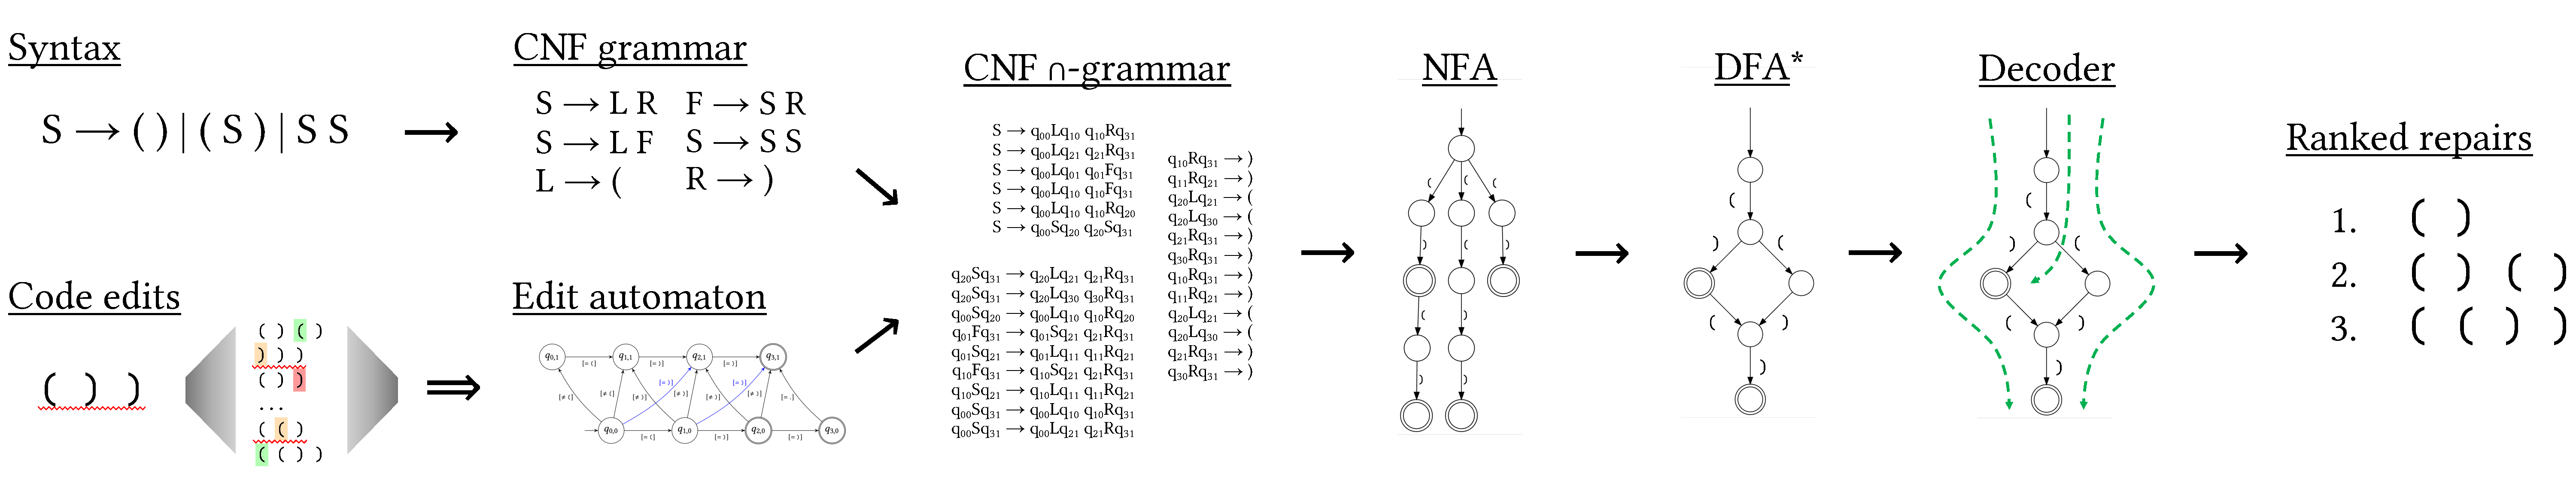
\includegraphics[width=\textwidth]{content/figures/flow.pdf}\vspace{-1pt}
  \caption{Simplified dataflow. Given a grammar and broken code fragment, we create an automaton generating the language of small edits, then construct a grammar representing the intersection of the two languages. This grammar can be converted to a finite automaton, determinized, then decoded to produce an explicit list of repairs.}\label{fig:arch_simp}
\end{figure}

The advantage of using this approach for syntax repair is that it performs the intersection not in the set domain, but in the domain of grammars and automata, thereby avoiding a great deal of useless work that would occur were we to compute the intersection by sampling and rejecting edits. Furthermore, it is a complete decision procedure, meaning that every possible repair within a given edit distance will eventually be found by the decoder.

To explain each component, we will require a more detailed background on the formal language theory, then we can describe the full Bar-Hillel construction and our specialization to Levenshtein automata intersections. But first, we will cover some related literature on program repair.

\clearpage
%\chapter*{\rm\bfseries Literature}
\label{ch:literature}

\mcgillguidelines: The comprehensive review of the literature must sufficiently demonstrate the student’s knowledge of and expertise in their research areas and should be broad enough to apply to each research question in the thesis. The review of the literature can additionally include various types of content, such as:

\begin{itemize}
    \item{A review providing a reader who is relatively less familiar with the research topic (e.g., an internal/external member of an oral defence committee with adjacent but not direct expertise) an introduction to the general domain.}
    \item{An explanation of the overall rationale for how and why the subsequent studies were conducted. For example, the literature underlying the research questions must be sufficiently discussed.}
    \item{A review of fundamental theories underlying the subsequently presented work, or to explain why certain approaches were not taken in the study(ies) presented.}
\end{itemize}

The literature review must be in line with disciplinary expectations. The review can be incorporated in the Introduction chapter, addressed in a standalone chapter, or distributed across multiple chapters.

% Two sample parts with sample chapters, change this parts as much as your little heart desires:
%\part{Why Does the Sun Shine?}
%\label{part:part1}
\chapter{\rm\bfseries Formal Language Theory}
\label{ch:chapter01}

In computer science, it is common to conflate two distinct notions for a set. The first is a collection sitting on some storage device, e.g., a dataset. The second is a lazy construction: not an explicit collection of objects, but a representation that allows us to efficiently determine membership on demand. This representation lets us describe infinite sets without requiring an infinite amount of storage. Inclusion then, instead of being simply a lookup query, becomes a decision procedure. This is the basis of formal language theory.

The representation we are chiefly interested in is called a \textit{grammar}, a common metanotation for specifying the syntactic constraints on programs, shared by nearly every programming language. Programming language grammars are overapproximations to the true language, but provide a reasonably detailed specification for rejecting invalid programs and parsing valid ones.

Formal languages are arranged in a hierarchy of containment, where each language family strictly contains its predecessors. On the lowest level of the hierarchy are finite languages. Type 3 contains finite and infinite languages generated by a regular grammar. Type 2 contains context-free languages, which admit parenthetical nesting. Supersets, such as the recursively enumerable sets, are Type 0. There are other kinds of formal languages, such as logics and circuits, which are incomparable with the Chomsky hierarchy.

Most programming languages leave level 2 after the parsing stage, and enter the realm of type theory. At this point, compiler authors layer additional semantic refinements on top of syntax, but must deal with phase ordering problems related to the sequencing of such analyzers, breaking commutativity and posing challenges for parallelization. This lack of compositionality is a major obstacle to the development of modular static analyses.

The advantage of dealing with formal language representations is that we can reason about them algebraically. Consider the context-free grammar: the arrow $\rightarrow$ becomes an $=$ sign, $\mid$ becomes $+$ and $AB$ becomes $A \times B$. The ambiguous Dyck grammar, then, can be seen as a system of equations.

\begin{equation}
    S \rightarrow ( ) \mid ( S ) \mid S S \Longleftrightarrow f(x) = x^2 + x^2 f(x) + f(x)^2
\end{equation}

\noindent We will now solve for $f(x)$, giving us the generating function for the language:

\begin{equation}
  0 = f(x)^2 + x^2 f(x) - f(x) + x^2
\end{equation}

\noindent Now, using the quadratic equation, where $a = 1, b = x^2 - 1, c = x^2$, we have:

\begin{equation}
  f(x) = \frac{-b \pm \sqrt{b^2 - 4ac}}{2a} = \frac{-x^2 + 1 \pm \sqrt{x^4 - 6x^2 + 1}}{2}
\end{equation}

\noindent Note there are two solutions, but only one where $\lim_{x\rightarrow 0} = 1$. From the ordinary generating function (OGF), we also have that $f(x)=\sum _{n=0}^{\infty }f_nx^{n}$. Expanding $\sqrt{x^4 - 6x^2 + 1}$ via the generalized binomial theorem, we have:

\begin{align}
f(x) = (1+u)^{\alpha }&=\sum _{k=0}^{\infty }\;{\binom {\alpha }{k}}\;u^{k}\\
  &=\sum _{k=0}^{\infty }\;{\binom {\frac{1}{2} }{k}}\;(x^4 - 6x^2)^{k} \text{ where } u = x^4-6x^2
\end{align}

Now, to obtain the number of ambiguous Dyck trees of size $n$, we can extract the $x^n$-th coefficient using the binomial series:

\begin{align}
  [x^n]f(x) &= [x^n]\frac{-x^2 + 1}{2} + \frac{1}{2}[x^n]\sum _{k=0}^{\infty }\;{\binom {\frac{1}{2} }{k}}\;(x^4 - 6x^2)^{k}\\
  [x^n]f(x) &= \frac{1}{2}{\binom {\frac{1}{2} }{n}}\;[x^n](x^4 - 6x^2)^n = \frac{1}{2}{\binom {\frac{1}{2} }{n}}\;[x^n](x^2 - 6x)^n
\end{align}

We can use this technique, first described by Flajolet \& Sedgewick~\cite{flajolet2009analytic}, to count the number of trees of a given size or distinct words in an unambiguous CFG. This lets us understand grammars as a kind of algebra, which is useful for enumerative combinatorics on words and syntax-guided synthesis.

Naturally, like algebra, there is also a kind of calculus to formal languages. Janusz Brzozowski~\cite{brzozowski1964derivatives} introduced the derivative operator for regular languages, which can be used to determine membership, and extract subwords from the language. This operator has been extended to CFLs by Might et al.~\cite{might2011parsing}, and is the basis for a family of elegant parsing algorithms.

The Brzozowski derivative has an extensional and intensional form. Extensionally, we have $\partial_a L = \{b \in \Sigma^* \mid ab \in L\}$. Intensionally, we have an induction over generalized regular expressions (GREs), which are a superset of regular expressions that supports intersection and negation.\vspace{-1cm}

\begin{multicols}{2}
  \begin{eqnarray*}
    \phantom{-}\partial_a( & \varnothing & )= \varnothing                                           \\
    \phantom{-}\partial_a( & \varepsilon & )= \varnothing                                           \\
    \phantom{-}\partial_a( & a           & )= \varepsilon                                           \\
    \phantom{-}\partial_a( & b           & )= \varnothing  \text{ for each } a \neq b               \\
    \phantom{-}\partial_a( & R^*         & )= (\partial_x R)\cdot R^*                               \\
    \phantom{-}\partial_a( & \neg R      & )= \neg \partial_a R                                     \\
    \phantom{-}\partial_a( & R\cdot S    & )= (\partial_a R)\cdot S \vee \delta(R)\cdot\partial_a S \\
    \phantom{-}\partial_a( & R\vee S     & )= \partial_a R \vee \partial_a S                        \\
    \phantom{-}\partial_a( & R\land S    & )= \partial_a R \land \partial_a S
  \end{eqnarray*} \break\vspace{-0.5cm}
  \begin{eqnarray*}
    \phantom{---}\delta(& \varnothing &)= \varnothing                                      \\
    \phantom{---}\delta(& \varepsilon &)= \varepsilon                                      \\
    \phantom{---}\delta(& a           &)= \varnothing                                      \\
    \phantom{---}\delta(& R^*         &)= \varepsilon                                      \\
    \phantom{---}\delta(& \neg R      &)= \varepsilon \text{ if } \delta(R) = \varnothing  \\
    \phantom{---}\delta(& \neg R      &)= \varnothing \text{ if } \delta(R) = \varepsilon  \\
    \phantom{---}\delta(& R\cdot S    &)= \delta(R) \land \delta(S)                        \\
    \phantom{---}\delta(& R\vee S     &)= \delta(R) \vee  \delta(S)                        \\
    \phantom{---}\delta(& R\land S    &)= \delta(R) \land \delta(S)
  \end{eqnarray*}
\end{multicols}

Similar to sets, it is possible to combine languages by manipulating their grammars, mirroring the setwise notions of union, intersection, complementation and difference over languages. These operations are convenient for combining, for example, syntactic and semantic constraints on programs. For example, we might have two grammars, $G_a, G_b$ representing two properties that are desirable or necessary for a program to be considered valid. %We can treat valid programs $P$ as a subset of the language intersection $P \subseteq \mathcal{L}(G_a) \cap \mathcal{L}(G_b)$.

Like all representations, grammars are themselves a trade-off between expressiveness and efficiency. It is possible to represent the same finite set with multiple representations of varying complexity. For example, the set of strings containing ten or fewer balanced parentheses can be expressed as a finite automaton containing millions of states, or a simple language conjunction containing a few productions, e.g., $\mathcal{L}\Big(S \rightarrow ( ) \mid (S) \mid S S \Big) \cap \Sigma^{[0,10]}$.

The choice of representation is heavily usage-dependent. For example, if we are interested in recognition, we might favor a disjoint representation, allowing properties to be checked independently without merging, whereas if we are interested in generation or deciding non-emptiness, we might prefer a unified representation which can be efficiently sampled without rejection.

Union, concatenation and repetition are all mundane in the theory of formal languages. Intersection and negation are more challenging concepts to borrow from set theory, and do not translate naturally into the Chomsky hierarchy. For example, the intersection of two CFLs is Turing Complete, but the intersection of a CFL and a regular language is a CFL.

Deciding intersection non-emptiness (INE) of a finite collection of finite automata is known to be PSPACE-complete~\cite{kozen1977lower}. It is still unknown whether a faster algorithm than the product construction exists for deciding INE of just two finite automata.

The textbook algorithm proceeds as follows: create an automaton containing the cross-product of states, and simulate both automata in lockstep, creating arcs between states that are co-reachable. If a final state is reachable in the product automaton, then the intersection is non-empty. This requires space proportional to the Cartesian product of the two states.

\begin{figure}[h]
  \caption{TODO: depict product construction for finite automata here.}
  \end{figure}

The goal of this thesis is to speed up the product construction by leveraging (1) parameterized complexity (2) pruning and (3) parallelization to speed up the wallclock runtime of the product construction and generalize it to CFG-REG intersections. We show it is possible to decide INE in realtime for intersections with Levenshtein automata and build a tool to demonstrate it on real-world programming languages and grammars.

Finally, we show a probabilistic extension of the REG-CFL product construction, which can be used to decode the top-K most probable words in the intersection of two formal languages. This is useful for languages with both formal and natural characteristics, where we might want to find the most natural word that satisfies multiple constraints, such as being a valid repair with fewer than $k$ edits whose probability is maximized.

\clearpage
\chapter{\rm\bfseries Deterministic Program Repair}
\label{ch:chapter02}

Parsimony is a guiding principle in program repair that comes from the 14th century Fransiscan friar named William of Ockham. In keeping with the Fransiscan minimalist lifestyle, Ockham's principle basically says that when you have multiple hypotheses, the simplest one is the best. It is not precisely clear what ``simple'' ought to mean in the context of program repair, but a first-order approximation is to strive for the smallest number of changes required to transform an invalid program into a valid one.

Levenshtein distance is one such metric for measuring the minimum number of changes between two strings. First proposed by the Soviet scientist Vladimir Levenshtein, it quantifies how many insertions, deletions, and substitutions are required to transform one string into another. Conveniently, there is an automaton, called the Levenshtein automaton~\cite{schulz2002fast}, that recognizes all strings within a given edit distance of a given string. We can use this automaton to locate the positions and contents of the most likely repair consistent with the observed program and the grammar.

The closure of CFLs under intersection with regular languages was first established in 1961 by Bar-Hillel, implying the existence of a context-free grammar representing the conjunction of any finite automaton and context-free grammar. Such a construction was given by Salomaa in 1973, who provides a direct, but inefficient, construction. In our work, we refine this construction to intersections with Levenshtein automata, which recognize all and only strings within a given edit distance of a reference string. Using this refinement, we demonstrate it is feasible to repair multiline syntax errors in practical programming languages.

\begin{wrapfigure}{r}{0.4\textwidth}
  \vspace{-0.2cm}
  \resizebox{0.42\textwidth}{!}{
  \def\secondcirclepath{(1.15,0) coordinate (e) circle (2cm)}
  \begin{tikzpicture}[
    dot/.style = {circle, inner sep=0pt, minimum size=1mm, fill,
    node contents={}}
  ]
    \def\firstcircle{(-2.1,0) coordinate (a) circle (2.4cm)}
    \def\firstcirclea{(-2.1,0) coordinate (b) circle (0.6cm)}
    \def\firstcircleb{(-2.1,0) coordinate (c) circle (1.2cm)}
    \def\firstcirclec{(-2.1,0) coordinate (d) circle (1.8cm)}
    \def\secondcircle{(1.2,0) coordinate (e) circle (1.5cm)}

    \begin{scope}
      \clip[decorate, decoration={snake, amplitude=0.6mm, segment length=5.01mm}] \secondcirclepath;
      \fill[black!35] \firstcircle;
    \end{scope}

    \draw \firstcircle node[dot,label=$\err{\sigma}$](z0);
    \draw [dashed] \firstcirclea;
    \draw [dashed] \firstcircleb;
    \draw [dashed] \firstcirclec;
    \draw[-stealth] (-2.1,0) -- (-1.5, 0) node[midway,below]{$d_1$};
    \draw[-stealth] (-1.5,0) -- (-0.9, 0) node[midway,below]{$d_2$};
    \draw[-stealth] (-0.9,0) -- (-0.3, 0) node[midway,below]{$d^*$};
    \draw[-stealth] (-0.3,0) -- (0.3, 0) node[midway,above]{$\tilde{\sigma}$};
    \draw[-stealth] (-0.3,0) -- (0.3, 0) node[midway,below]{$d^+$};

    \draw[decorate, decoration={snake, amplitude=0.6mm, segment length=5.01mm}] \secondcirclepath;
    \node [above] at (current bounding box.north -| a) {$\mathcal{L}\bigl(L(\err\sigma, d^*)\bigr)$};
    \node [above,yshift=2.1cm] at (e) {$\mathcal{L}(G)$};
  \end{tikzpicture}
}
  \vspace{-0.3cm}
  \caption{CFL intersection with the local edit region of a given broken code snippet.}
  \vspace{-0.2cm}
\end{wrapfigure}

Given the source code for a computer program $\err\sigma$ and a grammar $G$, our goal is to find every valid string $\sigma$ consistent with the grammar $G$ and within a certain edit distance, $d$. Consider the language of valid strings within a given Levenshtein distance from a reference string $\err\sigma$. We can intersect the language given by the Levenshtein automaton with the language of all valid programs given by the grammar $G$. The resulting language, $\mathcal{L}(G_\cap)$ will contain every repair within the designated edit distance.

\section{Levenshtein Automata}

Levenshtein automata are finite automata that recognize all and only strings within a given edit distance of another string by permitting insertions, deletions, and substitutions. For instance, suppose we have the input, \texttt{( ) )}, and wish to find nearby or parsimonious edits. To represent the language of parsimonious edits, we can construct the Levenshtein-1 automaton accepting every string that can be formed by inserting, substituting or deleting a single parenthesis. We depict this automaton in Figure~\ref{fig:lev_automaton}.

\begin{figure}[h!]
  \resizebox{0.45\textwidth}{!}{
  \begin{tikzpicture}[
%->, % makes the edges directed
    >=stealth',
    node distance=2.5cm, % specifies the minimum distance between two nodes. Change if necessary.
%  every state/.style={thick, fill=gray!10}, % sets the properties for each ’state’ node
    initial text=$ $, % sets the text that appears on the start arrow
  ]
    \node[state, initial]                (00) {$q_{0,0}$};
    \node[state, right of=00]            (10) {$q_{1,0}$};
    \node[accepting, state, right of=10] (20) {$q_{2,0}$};
    \node[accepting, state, right of=20] (30) {$q_{3,0}$};

    \node[state, above of=00, shift={(-2cm,0cm)}] (01) {$q_{0,1}$};
    \node[state, right of=01]                     (11) {$q_{1,1}$};
    \node[state, right of=11]                     (21) {$q_{2,1}$};
    \node[accepting, state, right of=21]          (31) {$q_{3,1}$};

    \draw [->] (00) edge[below] node{$\texttt{(}$} (10);
    \draw [->] (10) edge[below] node{$\texttt{)}$} (20);
    \draw [->] (20) edge[below] node{$\texttt{)}$} (30);

    \draw [->] (01) edge[below] node{$\texttt{(}$}                       (11);
    \draw [->] (11) edge[below] node[shift={(-0.2cm,0cm)}]{$\texttt{)}$} (21);
    \draw [->] (21) edge[below] node[shift={(-0.2cm,0cm)}]{$\texttt{)}$} (31);

    \draw [->] (00) edge[bend left=10] node[shift={(-0.15cm,0cm)}]{\tiny{$\texttt{(}$}} (11);
    \draw [->] (10) edge[bend left=10] node[shift={(-0.15cm,0cm)}]{\tiny{$\texttt{(}$}} (21);
    \draw [->] (20) edge[bend left=10] node[shift={(-0.15cm,0cm)}]{\tiny{$\texttt{(}$}} (31);

    \draw [->] (00) edge[bend left=10, left] node[shift={(-0.1cm,0cm)}]{\tiny{$\texttt{(}$}} (01);
    \draw [->] (10) edge[bend left=10, left] node[shift={(-0.1cm,0cm)}]{\tiny{$\texttt{(}$}} (11);
    \draw [->] (20) edge[bend left=10, left] node[shift={(-0.1cm,0cm)}]{\tiny{$\texttt{(}$}} (21);

    \draw [->] (00) edge[bend right=10, right] node{\tiny{$\texttt{)}$}} (11);
    \draw [->] (10) edge[bend right=10, right] node{\tiny{$\texttt{)}$}} (21);
    \draw [->] (20) edge[bend right=10, right] node{\tiny{$\texttt{)}$}} (31);

    \draw [->] (00) edge[bend right=10, right] node{\tiny{$\texttt{)}$}} (01);
    \draw [->] (10) edge[bend right=10, right] node{\tiny{$\texttt{)}$}} (11);
    \draw [->] (20) edge[bend right=10, right] node{\tiny{$\texttt{)}$}} (21);

    \draw [->] (30) edge[bend left=10, left] node[shift={(-0.1cm,0cm)}]{\tiny{$\texttt{(}$}} (31);
    \draw [->] (30) edge[bend right=10, right] node{\tiny{$\texttt{)}$}} (31);

    \draw [->, blue] (00) edge[bend right=11,below] node[shift={(0.4cm,0.9cm)}]{$\texttt{)}$}    (21);
    \draw [->, blue] (10) edge[bend right=11,below] node[shift={(0.4cm,0.9cm)}]{$\texttt{)}$}    (31);
    \node[align=center, yshift=2em, xshift=-1cm] (title) at (current bounding box.north) {Original Levenshtein automaton};
  \end{tikzpicture}
}
\resizebox{0.515\textwidth}{!}{
  \begin{tikzpicture}[
%->, % makes the edges directed
    >=stealth',
    node distance=2.5cm, % specifies the minimum distance between two nodes. Change if necessary.
%  every state/.style={thick, fill=gray!10}, % sets the properties for each ’state’ node
    initial text=$ $, % sets the text that appears on the start arrow
  ]
    \draw[orange,->] (-4cm,1.2cm) -- (-3cm,1.2cm);

    \node[state, initial]                (00) {$q_{0,0}$};
    \node[state, right of=00]            (10) {$q_{1,0}$};
    \node[accepting, state, right of=10] (20) {$q_{2,0}$};
    \node[accepting, state, right of=20] (30) {$q_{3,0}$};

    \node[state, above of=00, shift={(-2cm,0cm)}] (01) {$q_{0,1}$};
    \node[state, right of=01]                     (11) {$q_{1,1}$};
    \node[state, right of=11]                     (21) {$q_{2,1}$};
    \node[accepting, state, right of=21]          (31) {$q_{3,1}$};

    \draw [->] (00) edge[below] node{\tiny{$[= \texttt{(}]$}} (10);
    \draw [->] (10) edge[below] node{\tiny{$[= \texttt{)}]$}} (20);
    \draw [->] (20) edge[below] node{\tiny{$[= \texttt{)}]$}} (30);

    \draw [->] (01) edge[below] node{\tiny{$[= \texttt{(}]$}}                       (11);
    \draw [->] (11) edge[below] node[shift={(-0.2cm,0cm)}]{\tiny{$[= \texttt{)}]$}} (21);
    \draw [->] (21) edge[below] node[shift={(-0.2cm,0cm)}]{\tiny{$[= \texttt{)}]$}} (31);

    \draw [->] (00) edge[left] node{\tiny{$[\neq \texttt{(}]$}} (11);
    \draw [->] (10) edge[left] node{\tiny{$[\neq \texttt{)}]$}} (21);
    \draw [->] (20) edge[left] node{\tiny{$[\neq \texttt{)}]$}} (31);

    \draw [->] (00) edge[bend left=10, left] node{\tiny{$[\neq \texttt{(}]$}} (01);
    \draw [->] (10) edge[bend left=10, left] node{\tiny{$[\neq \texttt{)}]$}} (11);
    \draw [->] (20) edge[bend left=10, left] node{\tiny{$[\neq \texttt{)}]$}} (21);
    \draw [->] (30) edge[bend left=10, left] node{\tiny{$[=.]$}} (31);


    \draw [->, blue] (00) edge[bend right=11,below] node[shift={(0.2cm,0.8cm)}]{\tiny{$[= \texttt{)}]$}}    (21);
    \draw [->, blue] (10) edge[bend right=11,below] node[shift={(0.2cm,0.8cm)}]{\tiny{$[= \texttt{)}]$}}    (31);
    \node[align=center, yshift=2em, xshift=-0.4cm] (title) at (current bounding box.north) {Nominal Levenshtein automaton (ours)};
  \end{tikzpicture}
}
  \caption{Automaton recognizing every 1-edit patch. We nominalize the original automaton, ensuring upward arcs denote a mutation, and use a symbolic predicate, which deduplicates parallel arcs in large alphabets.}\label{fig:lev_automaton}\vspace{-5pt}
\end{figure}

The original automaton is nondeterministic, containing an upward arc for each token. This can be avoided with a simple modification that matches an inequality predicate. The machine enters at $q_{0, 0}$ and at each step, accepts the labeled token. Final states are encircled twice, denoting that any trajectory ending at such a state is considered valid.
When the edit distance grows larger, we introduce some additional arcs to handle multi-token deletions, but the overall picture remains unchanged. We depict a 3x5 automaton recognizing 3-edit patches of a length-5 string in Figure~\ref{fig:lev_nfa}.

\begin{figure}%{r}{0.4\textwidth}
  \begin{center}
      \resizebox{0.8\textwidth}{!}{
  \begin{tikzpicture}[
%->, % makes the edges directed
  >=stealth',
  node distance=2.5cm, % specifies the minimum distance between two nodes. Change if necessary.
%  every state/.style={thick, fill=gray!10}, % sets the properties for each ’state’ node
  initial text=$ $, % sets the text that appears on the start arrow
  ]
  \node[state, initial]                (00) {$q_{0,0}$};
  \node[state, right of=00]            (10) {$q_{1,0}$};
  \node[accepting, state, right of=10] (20) {$q_{2,0}$};
  \node[accepting, state, right of=20] (30) {$q_{3,0}$};
  \node[accepting, state, right of=30] (40) {$q_{4,0}$};
  \node[accepting, state, right of=40] (50) {$q_{5,0}$};

  \node[state, above of=00, shift={(-2cm,0cm)}] (01) {$q_{0,1}$};
  \node[state, right of=01]                          (11) {$q_{1,1}$};
  \node[state, right of=11]                          (21) {$q_{2,1}$};
  \node[accepting, state, right of=21]               (31) {$q_{3,1}$};
  \node[accepting, state, right of=31]               (41) {$q_{4,1}$};
  \node[accepting, state, right of=41]               (51) {$q_{5,1}$};

\node[state, above of=01, shift={(-2cm,0cm)}] (0j) {$q_{0,2}$};
\node[state, right of=0j]                          (1j) {$q_{1,2}$};
\node[state, right of=1j]                          (2j) {$q_{2,2}$};
\node[state, right of=2j]                          (3j) {$q_{3,2}$};
\node[accepting, state, right of=3j]               (4j) {$q_{4,2}$};
\node[accepting, state, right of=4j]               (5j) {$q_{5,2}$};

\node[state, above of=0j, shift={(-2cm,0cm)}] (0k) {$q_{0,3}$};
\node[state, right of=0k]                         (1k) {$q_{1,3}$};
\node[state, right of=1k]                         (2k) {$q_{2,3}$};
\node[state, right of=2k]                         (3k) {$q_{3,3}$};
\node[state, right of=3k]                         (4k) {$q_{4,3}$};
\node[accepting, state, right of=4k]              (5k) {$q_{5,3}$};

\draw [->] (00) edge[below] node{$\sigma_1$} (10);
\draw [->] (10) edge[below] node{$\sigma_2$} (20);
\draw [->] (20) edge[below] node{$\sigma_3$} (30);
\draw [->] (30) edge[below] node{$\sigma_4$} (40);
\draw [->] (40) edge[below] node{$\sigma_5$} (50);

\draw [->] (01) edge[below] node{$\sigma_1$} (11);
\draw [->] (11) edge[below] node[shift={(-0.2cm,0cm)}]{$\sigma_2$} (21);
\draw [->] (21) edge[below] node[shift={(-0.2cm,0cm)}]{$\sigma_3$} (31);
\draw [->] (31) edge[below] node[shift={(-0.2cm,0cm)}]{$\sigma_4$} (41);
\draw [->] (41) edge[below] node{$\sigma_5$} (51);

\draw [->] (0j) edge[below] node{$\sigma_1$} (1j);
\draw [->] (1j) edge[below] node{$\sigma_2$} (2j);
\draw [->] (2j) edge[below] node{$\sigma_3$} (3j);
\draw [->] (3j) edge[below] node{$\sigma_4$} (4j);
\draw [->] (4j) edge[below] node{$\sigma_5$} (5j);

\draw [->] (0k) edge[below] node{$\sigma_1$} (1k);
\draw [->] (1k) edge[below] node{$\sigma_2$} (2k);
\draw [->] (2k) edge[below] node{$\sigma_3$} (3k);
\draw [->] (3k) edge[below] node{$\sigma_4$} (4k);
\draw [->] (4k) edge[below] node{$\sigma_5$} (5k);

\draw [->] (00) edge[left] node{$\phantom{\cdot}$} (11);
\draw [->] (10) edge[left] node{$\phantom{\cdot}$} (21);
\draw [->] (20) edge[left] node{$\phantom{\cdot}$} (31);
\draw [->] (30) edge[left] node{$\phantom{\cdot}$} (41);
\draw [->] (40) edge[left] node{$\phantom{\cdot}$} (51);

% Super-knight arcs
\draw [->, red] (00) edge[bend right=8] node[east, shift={(-0.2cm,-0.7cm)}]{$\color{red}\sigma_3$}         (3j);
\draw [->, red] (10) edge[bend right=8] node[east, shift={(-0.2cm,-0.7cm)}]{$\color{red}\sigma_4$}         (4j);
\draw [->, red] (20) edge[bend right=8] node[east, shift={(-0.2cm,-0.7cm)}]{$\color{red}\sigma_5$}         (5j);

\draw [->, red] (01) edge[bend left=8] node[east, shift={(-0.2cm,-0.7cm)}]{$\color{red}\sigma_3$}         (3k);
\draw [->, red] (11) edge[bend left=8] node[east, shift={(-0.2cm,-0.7cm)}]{$\color{red}\sigma_4$}         (4k);
\draw [->, red] (21) edge[bend left=8] node[east, shift={(-0.2cm,-0.7cm)}]{$\color{red}\sigma_5$}         (5k);

\draw [->, violet] (00) edge node[east, shift={(-0.1cm,-0.8cm)}]{$\color{violet}\sigma_4$}  (4k);
\draw [->, violet] (10) edge node[east, shift={(-0.1cm,-0.8cm)}]{$\color{violet}\sigma_5$}  (5k);

\draw [->] (01) edge[left] node{$\phantom{\cdot}$} (1j);
\draw [->] (11) edge[left] node{$\phantom{\cdot}$} (2j);
\draw [->] (21) edge[left] node{$\phantom{\cdot}$} (3j);
\draw [->] (31) edge[left] node{$\phantom{\cdot}$} (4j);
\draw [->] (41) edge[left] node{$\phantom{\cdot}$} (5j);

\draw [->] (0j) edge[left] node{$\phantom{\cdot}$} (1k);
\draw [->] (1j) edge[left] node{$\phantom{\cdot}$} (2k);
\draw [->] (2j) edge[left] node{$\phantom{\cdot}$} (3k);
\draw [->] (3j) edge[left] node{$\phantom{\cdot}$} (4k);
\draw [->] (4j) edge[left] node{$\phantom{\cdot}$} (5k);

\draw [->] (00) edge[bend left=10, left] node{$\phantom{\cdot}$} (01);
\draw [->] (10) edge[bend left=10, left] node{$\phantom{\cdot}$} (11);
\draw [->] (20) edge[bend left=10, left] node{$\phantom{\cdot}$} (21);
\draw [->] (30) edge[bend left=10, left] node{$\phantom{\cdot}$} (31);
\draw [->] (40) edge[bend left=10, left] node{$\phantom{\cdot}$} (41);
\draw [->] (50) edge[bend left=10, left] node{$\phantom{\cdot}$} (51);

\draw [->] (01) edge[bend left=10, left] node{$\phantom{\cdot}$} (0j);
\draw [->] (11) edge[bend left=10, left] node{$\phantom{\cdot}$} (1j);
\draw [->] (21) edge[bend left=10, left] node{$\phantom{\cdot}$} (2j);
\draw [->] (31) edge[bend left=10, left] node{$\phantom{\cdot}$} (3j);
\draw [->] (41) edge[bend left=10, left] node{$\phantom{\cdot}$} (4j);
\draw [->] (51) edge[bend left=10, left] node{$\phantom{\cdot}$} (5j);

\draw [->] (0j) edge[bend left=10, left] node{$\phantom{\cdot}$} (0k);
\draw [->] (1j) edge[bend left=10, left] node{$\phantom{\cdot}$} (1k);
\draw [->] (2j) edge[bend left=10, left] node{$\phantom{\cdot}$} (2k);
\draw [->] (3j) edge[bend left=10, left] node{$\phantom{\cdot}$} (3k);
\draw [->] (4j) edge[bend left=10, left] node{$\phantom{\cdot}$} (4k);
\draw [->] (5j) edge[bend left=10, left] node{$\phantom{\cdot}$} (5k);

\draw [->, blue] (00) edge[bend right=11,below] node[shift={(0.5cm,0.3cm)}]{$\color{blue}\sigma_2$}    (21);
\draw [->, blue] (10) edge[bend right=11,below] node[shift={(0.5cm,0.3cm)}]{$\color{blue}\sigma_3$}    (31);
\draw [->, blue] (20) edge[bend right=11,below] node[shift={(0.5cm,0.3cm)}]{$\color{blue}\sigma_4$}    (41);
\draw [->, blue] (30) edge[bend right=11,below] node[shift={(0.5cm,0.3cm)}]{$\color{blue}\sigma_5$}    (51);

\draw [->, blue] (01) edge[bend right=3,below] node[shift={(0.3cm,0.2cm)}]{$\color{blue}\sigma_2$}    (2j);
\draw [->, blue] (11) edge[bend right=3,below] node[shift={(0.3cm,0.2cm)}]{$\color{blue}\sigma_3$}    (3j);
\draw [->, blue] (21) edge[bend right=3,below] node[shift={(0.3cm,0.2cm)}]{$\color{blue}\sigma_4$}    (4j);
\draw [->, blue] (31) edge[bend right=3,below] node[shift={(0.3cm,0.2cm)}]{$\color{blue}\sigma_4$}    (5j);

\draw [->, blue] (0j) edge[bend left=8,below] node[shift={(-0.45cm,-0.55cm)}]{$\color{blue}\sigma_2$}    (2k);
\draw [->, blue] (1j) edge[bend left=8,below] node[shift={(-0.45cm,-0.55cm)}]{$\color{blue}\sigma_3$}    (3k);
\draw [->, blue] (2j) edge[bend left=8,below] node[shift={(-0.45cm,-0.55cm)}]{$\color{blue}\sigma_4$}    (4k);
\draw [->, blue] (3j) edge[bend left=8,below] node[shift={(-0.45cm,-0.55cm)}]{$\color{blue}\sigma_5$}    (5k);

%https://tex.stackexchange.com/a/20986/139648
\draw [decorate,decoration={brace,amplitude=10pt,raise=10pt,mirror}] (00.south west) -- (50.south east) node[midway,yshift=-3em]{\textbf{String length}};
\draw [decorate,decoration={brace,amplitude=10pt,raise=20pt}] (00.south west) -- (0k.north west) node[midway,xshift=-1cm,yshift=-1cm,rotate=-54]{\textbf{Edit distance}};
\end{tikzpicture}
}
  \end{center}
  \caption{NFA recognizing Levenshtein $L(\sigma: \Sigma^5, 3)$.}\label{fig:lev_nfa}
\end{figure}

Here, a pattern begins to emerge: the automaton is a grid of states, with each horizontal arc consuming a token in the original string, and upwards arcs recognizing mutations. Traversing a vertical arc corresponds to an insertion or substitution, and a diagonal arc corresponds to a deletion. Levenshtein automata can also be defined as a set of inference rules, which generalize this picture to arbitrary length strings and edit distances. The indices are a bit finicky, but the rules are otherwise straightforward.

\begin{prooftree}
  \AxiomC{$s\in\Sigma \phantom{\land} i \in [0, n] \phantom{\land} j \in [1, d_{\max}]$}
  \RightLabel{$\duparrow$}
  \UnaryInfC{$(q_{i, j-1} \overset{s}{\rightarrow} q_{i,j}) \in \delta$}
  \DisplayProof
  \hskip 1.5em
  \AxiomC{$s\in\Sigma \phantom{\land} i \in [1, n] \phantom{\land} j \in [1, d_{\max}]$}
  \RightLabel{$\ddiagarrow$}
  \UnaryInfC{$(q_{i-1, j-1} \overset{s}{\rightarrow} q_{i,j}) \in \delta$}
\end{prooftree}
\begin{prooftree}
  \AxiomC{$i \in [1, n] \phantom{\land} j \in [0, d_{\max}]$}
  \RightLabel{$\drightarrow$}
  \UnaryInfC{$(q_{i-1, j} \overset{\sigma_i}{\rightarrow} q_{i,j}) \in \delta$}
  \DisplayProof
  \hskip 1.5em
  \AxiomC{$d \in [1, d_{\max}] \phantom{\land} i \in [d + 1, n] \phantom{\land} j \in [d, d_{\max}]$}
  \RightLabel{$\knightarrow$}
  \UnaryInfC{$(q_{i-d-1, j-d} \overset{\sigma_i}{\rightarrow} q_{i,j}) \in \delta$}
\end{prooftree}
\begin{prooftree}
  \AxiomC{$\vphantom{|}$}
  \RightLabel{$\textsc{Init}$}
  \UnaryInfC{$q_{0,0} \in I$}
  \DisplayProof
  \hskip 1.5em
  \AxiomC{$q_{i, j} \in Q$}
  \AxiomC{$|n-i+j| \leq d_{\max}$}
  \RightLabel{$\textsc{Done}$}
  \BinaryInfC{$q_{i, j}\in F$}
\end{prooftree}


\newcommand{\substitutionExample}{
  \tikz{
    \foreach \x in {0,8,16,24,32,40}{
      \fill (\x pt,0pt) circle [radius = 1pt];
      \fill (\x pt,8pt) circle [radius = 1pt];
    }
    \phantom{\fill (0pt,-8pt) circle [radius = 1pt];}
    \draw [-to] (0pt,0pt) -- (8pt,0pt);
    \draw [-to] (8pt,0pt) -- (16pt,0pt);
    \draw [-to] (16pt,0pt) -- (24pt,8pt);
    \draw [-to] (24pt,8pt) -- (32pt,8pt);
    \draw [-to] (32pt,8pt) -- (40pt,8pt);
  }
}

\newcommand{\insertionExample}{
  \tikz{
    \foreach \x in {0,8,16,24,32,40}{
      \fill (\x pt,0pt) circle [radius = 1pt];
      \fill (\x pt,8pt) circle [radius = 1pt];
    }
    \phantom{\fill (0pt,-8pt) circle [radius = 1pt];}
    \fill[white] (16pt,0pt) circle [radius = 1.2pt];
    \fill[white] (24pt,8pt) circle [radius = 1.2pt];
    \draw [-to] (0pt,0pt) -- (8pt,0pt);
    \draw [-to] (8pt,0pt) -- (24pt,0pt);
    \draw [-to] (24pt,0pt) -- (16pt,8pt);
    \draw [-to] (16pt,8pt) -- (32pt,8pt);
    \draw [-to] (32pt,8pt) -- (40pt,8pt);
  }
}

\newcommand{\deletionExample}{
  \tikz{
    \foreach \x in {0,8,16,24,32,40}{
      \fill (\x pt,0pt) circle [radius = 1pt];
      \fill (\x pt,8pt) circle [radius = 1pt];
    }
    \phantom{\fill (0pt,-8pt) circle [radius = 1pt];}
    \draw [-to] (0pt,0pt) -- (8pt,0pt);
    \draw [-to] (8pt,0pt) -- (16pt,0pt);
    \draw [-to] (16pt,0pt) -- (24pt,0pt);
    \draw [-to] (24pt,0pt) -- (40pt,8pt);
  }
}

\newcommand{\doubleDeletionExample}{
  \tikz{
    \foreach \x in {0,8,16,24,32,40}{
      \fill (\x pt,0pt) circle [radius = 1pt];
      \fill (\x pt,8pt) circle [radius = 1pt];
      \fill (\x pt,16pt) circle [radius = 1pt];
    }
    \draw [-to] (0pt,0pt) -- (24pt,16pt);
    \draw [-to] (24pt,16pt) -- (32pt,16pt);
    \draw [-to] (32pt,16pt) -- (40pt,16pt);
  }
}

\newcommand{\subDelExample}{
  \tikz{
    \foreach \x in {0,8,16,24,32,40}{
      \fill (\x pt,0pt) circle [radius = 1pt];
      \fill (\x pt,8pt) circle [radius = 1pt];
      \fill (\x pt,16pt) circle [radius = 1pt];
    }
    \draw [-to] (0pt,0pt) -- (8pt,0pt);
    \draw [-to] (8pt,0pt) -- (16pt,8pt);
    \draw [-to] (16pt,8pt) -- (32pt,16pt);
    \draw [-to] (32pt,16pt) -- (40pt,16pt);
  }
}

\newcommand{\subSubExample}{
  \tikz{
    \foreach \x in {0,8,16,24,32,40}{
      \fill (\x pt,0pt) circle [radius = 1pt];
      \fill (\x pt,8pt) circle [radius = 1pt];
      \fill (\x pt,16pt) circle [radius = 1pt];
    }
    \draw [-to] (0pt,0pt) -- (8pt,0pt);
    \draw [-to] (8pt,0pt) -- (16pt,8pt);
    \draw [-to] (16pt,8pt) -- (24pt,16pt);
    \draw [-to] (24pt,16pt) -- (32pt,16pt);
    \draw [-to] (32pt,16pt) -- (40pt,16pt);
  }
}

\newcommand{\insertDeleteExample}{
  \tikz{
    \foreach \x in {0,8,16,24,32,40,48}{
      \fill (\x pt,0pt) circle [radius = 1pt];
      \fill (\x pt,8pt) circle [radius = 1pt];
      \fill (\x pt,16pt) circle [radius = 1pt];
    }
    \fill[white] (16pt,16pt) circle [radius = 1.2pt];
    \fill[white] (8pt,0pt) circle [radius = 1.2pt];
    \fill[white] (16pt,8pt) circle [radius = 1.2pt];
    \draw [-to] (0pt,0pt) -- (16pt,0pt);
    \draw [-to] (16pt,0pt) -- (8pt,8pt);
    \draw [-to] (8pt,8pt) -- (24pt,8pt);
    \draw [-to] (24pt,8pt) -- (40pt,16pt);
    \draw [-to] (40pt,16pt) -- (48pt,16pt);
  }
}

Each rule recognizes a specific type of edit. $\duparrow$ handles insertions, $\ddiagarrow$ handles substitutions and $\knightarrow$ handles deletions of one or more terminals. Let us consider some illustrative cases depicting the edit trajectory with specific Levenshtein alignments. Note that the trajectory may not be unique.

\begin{table}[H]
  \begin{tabular}{ccccccc}

    \texttt{f\hspace{3pt}.\hspace{3pt}\hlorange{[}\hspace{3pt}x\hspace{3pt})} &
    \texttt{f\hspace{3pt}.\hspace{3pt}\phantom{(}\hspace{3pt}x\hspace{3pt})} &
    \texttt{f\hspace{3pt}.\hspace{3pt}(\hspace{3pt}\hlred{x}\hspace{3pt})} &
    \texttt{\hlred{.}\hspace{3pt}\hlred{+}\hspace{3pt}(\hspace{3pt}x\hspace{3pt})} &
    \texttt{f\hspace{3pt}\hlorange{.}\hspace{3pt}\hlred{(}\hspace{3pt}x\hspace{3pt};} &
    \texttt{[\hspace{3pt}\hlorange{,}\hspace{3pt}\hlorange{x}\hspace{3pt}y\hspace{3pt}]} &
    \texttt{[\hspace{3pt}\phantom{,}\hspace{3pt},\hspace{3pt}\hlred{x}\hspace{3pt}y\hspace{3pt}]} \\

    \texttt{f\hspace{3pt}.\hspace{3pt}\hlorange{(}\hspace{3pt}x\hspace{3pt})} &
    \texttt{f\hspace{3pt}.\hspace{3pt}\hlgreen{(}\hspace{3pt}x\hspace{3pt})} &
    \texttt{f\hspace{3pt}.\hspace{3pt}(\hspace{3pt}\phantom{x}\hspace{3pt})} &
    \texttt{\phantom{f}\hspace{3pt}\phantom{.}\hspace{3pt}(\hspace{3pt}x\hspace{3pt})} &
    \texttt{f\hspace{3pt}\hlorange{*}\hspace{3pt}\phantom{(}\hspace{3pt}x\hspace{3pt};} &
    \texttt{[\hspace{3pt}\hlorange{x}\hspace{3pt}\hlorange{,}\hspace{3pt}y\hspace{3pt}]} &
    \texttt{[\hspace{3pt}\hlgreen{x}\hspace{3pt},\hspace{3pt}\phantom{x}\hspace{3pt}y\hspace{3pt}]} \\

    \substitutionExample & \insertionExample & \deletionExample & \doubleDeletionExample & \subDelExample & \subSubExample & \insertDeleteExample
  \end{tabular}
\end{table}

\section{The Bar-Hillel Construction}

The Bar-Hillel construction is a method for conjoining a context-free grammar with a finite automaton. First proposed by Bar-Hillel in 1961, and later realized by Salomaa in 1973, this construction is based on the idea of a product automaton, generalized to a grammar. It consists of three rules:

\begin{prooftree}
  \AxiomC{$q \in I \phantom{\land} r \in F\vphantom{\overset{a}{\rightarrow}}$}
  \RightLabel{$\sqrt{\phantom{S}}$}
  \UnaryInfC{$\big(S\rightarrow q S r\big) \in P_\cap$}
  \DisplayProof
  \hskip 1em
  \AxiomC{$(A \rightarrow a) \in P$}
  \AxiomC{$(q\overset{a}{\rightarrow}r) \in \delta$}
  \RightLabel{$\uparrow$}
  \BinaryInfC{$\big(qAr\rightarrow a\big)\in P_\cap$}
\end{prooftree}

\begin{prooftree}
  \AxiomC{$(w \rightarrow xz) \in P\vphantom{\overset{a}{\rightarrow}}$}
  \AxiomC{$p,q,r \in Q$}
  \RightLabel{$\Join$}
  \BinaryInfC{$\big(pwr\rightarrow (pxq)(qzr)\big) \in P_\cap$}
\end{prooftree}

\subsection{State elimination}

The $\Join$ rule has a strong dependency on the number of states. So, the primary target is to first reduce the number of states in the Levenshtein automaton. We can reduce the number of states without compromising the integrity of the Bar-Hillel construction by pruning states which are obviously inaccessible. For example, let us consider the following scenario, where $G = S \rightarrow \texttt{( } S \texttt{ )} \mid \texttt{[ } S \texttt{ ]} \mid S \texttt{ + } S \mid \texttt{1}$ and $\err{\sigma} = \texttt{[ ( + ) ]}$. If we can establish $\mathcal{L}(\texttt{\_ \_ + ) ]}) = \varnothing \land \mathcal{L}(\texttt{\_ \_ \_ ) ]})\neq \varnothing$ and $\mathcal{L}(\texttt{[ ( + \_ \_}) = \varnothing \land \mathcal{L}(\texttt{[ ( \_ \_ \_})\neq\varnothing$, then:

\begin{figure}[H]
  \begin{center}
     \resizebox{0.7\textwidth}{!}{
      \begin{tikzpicture}[
%->, % makes the edges directed
        >=stealth',
        node distance=2.5cm, % specifies the minimum distance between two nodes. Change if necessary.
%  every state/.style={thick, fill=gray!10}, % sets the properties for each ’state’ node
        initial text=$ $, % sets the text that appears on the start arrow
      ]
        \node[state, initial]                (00) {$q_{0,0}$};
        \node[state, right of=00]            (10) {$q_{1,0}$};
        \node[accepting, state, right of=10] (20) {$q_{2,0}$};
        \phantom{\node[accepting, state, right of=20] (30) {$q_{3,0}$};}
        \phantom{\node[accepting, state, right of=30] (40) {$q_{4,0}$};}
        \phantom{\node[accepting, state, right of=40] (50) {$q_{5,0}$};}

        \node[state, above of=00, shift={(-2cm,0cm)}] (01) {$q_{0,1}$};
        \node[state, right of=01]                          (11) {$q_{1,1}$};
        \node[state, right of=11]                          (21) {$q_{2,1}$};
        \node[accepting, state, right of=21]               (31) {$q_{3,1}$};
        \node[accepting, state, right of=31]               (41) {$q_{4,1}$};
        \node[accepting, state, right of=41]               (51) {$q_{5,1}$};

        \node[state, above of=01, shift={(-2cm,0cm)}] (0j) {$q_{0,2}$};
        \node[state, right of=0j]                          (1j) {$q_{1,2}$};
        \node[state, right of=1j]                          (2j) {$q_{2,2}$};
        \node[state, right of=2j]                          (3j) {$q_{3,2}$};
        \node[accepting, state, right of=3j]               (4j) {$q_{4,2}$};
        \node[accepting, state, right of=4j]               (5j) {$q_{5,2}$};

        \phantom{\node[state, above of=0j, shift={(-2cm,0cm)}] (0k) {$q_{0,3}$};}
        \phantom{\node[state, right of=0k]                         (1k) {$q_{1,3}$};}
        \phantom{\node[state, right of=1k]                         (2k) {$q_{2,3}$};}
        \node[state, right of=2k]                         (3k) {$q_{3,3}$};
        \node[state, right of=3k]                         (4k) {$q_{4,3}$};
        \node[accepting, state, right of=4k]              (5k) {$q_{5,3}$};

        \draw [->] (00) edge[below] node{$\sigma_1$} (10);
        \draw [->] (10) edge[below] node{$\sigma_2$} (20);
%        \draw [->] (20) edge[below] node{$\sigma_3$} (30);
%        \draw [->] (30) edge[below] node{$\sigma_4$} (40);
%        \draw [->] (40) edge[below] node{$\sigma_5$} (50);

        \draw [->] (01) edge[below] node{$\sigma_1$} (11);
        \draw [->] (11) edge[below] node[shift={(-0.2cm,0cm)}]{$\sigma_2$} (21);
        \draw [->] (21) edge[below] node[shift={(-0.2cm,0cm)}]{$\sigma_3$} (31);
        \draw [->] (31) edge[below] node[shift={(-0.2cm,0cm)}]{$\sigma_4$} (41);
        \draw [->] (41) edge[below] node{$\sigma_5$} (51);

        \draw [->] (0j) edge[below] node{$\sigma_1$} (1j);
        \draw [->] (1j) edge[below] node{$\sigma_2$} (2j);
        \draw [->] (2j) edge[below] node{$\sigma_3$} (3j);
        \draw [->] (3j) edge[below] node{$\sigma_4$} (4j);
        \draw [->] (4j) edge[below] node{$\sigma_5$} (5j);

%        \draw [->] (0k) edge[below] node{$\sigma_1$} (1k);
%        \draw [->] (1k) edge[below] node{$\sigma_2$} (2k);
%        \draw [->] (2k) edge[below] node{$\sigma_3$} (3k);
        \draw [->] (3k) edge[below] node{$\sigma_4$} (4k);
        \draw [->] (4k) edge[below] node{$\sigma_5$} (5k);

        \draw [->] (00) edge[left] node{$\phantom{\cdot}$} (11);
        \draw [->] (10) edge[left] node{$\phantom{\cdot}$} (21);
        \draw [->] (20) edge[left] node{$\phantom{\cdot}$} (31);
%        \draw [->] (30) edge[left] node{$\phantom{\cdot}$} (41);
%        \draw [->] (40) edge[left] node{$\phantom{\cdot}$} (51);

% Super-knight arcs
        \draw [->, red] (00) edge[bend right=8] node[east, shift={(-0.2cm,-0.7cm)}]{$\color{red}\sigma_3$}         (3j);
        \draw [->, red] (10) edge[bend right=8] node[east, shift={(-0.2cm,-0.7cm)}]{$\color{red}\sigma_4$}         (4j);
        \draw [->, red] (20) edge[bend right=8] node[east, shift={(-0.2cm,-0.7cm)}]{$\color{red}\sigma_5$}         (5j);

        \draw [->, red] (01) edge[bend left=8] node[east, shift={(-0.2cm,-0.7cm)}]{$\color{red}\sigma_3$}         (3k);
        \draw [->, red] (11) edge[bend left=8] node[east, shift={(-0.2cm,-0.7cm)}]{$\color{red}\sigma_4$}         (4k);
        \draw [->, red] (21) edge[bend left=8] node[east, shift={(-0.2cm,-0.7cm)}]{$\color{red}\sigma_5$}         (5k);

        \draw [->, violet] (00) edge node[east, shift={(-0.1cm,-0.8cm)}]{$\color{violet}\sigma_4$}  (4k);
        \draw [->, violet] (10) edge node[east, shift={(-0.1cm,-0.8cm)}]{$\color{violet}\sigma_5$}  (5k);

        \draw [->] (01) edge[left] node{$\phantom{\cdot}$} (1j);
        \draw [->] (11) edge[left] node{$\phantom{\cdot}$} (2j);
        \draw [->] (21) edge[left] node{$\phantom{\cdot}$} (3j);
        \draw [->] (31) edge[left] node{$\phantom{\cdot}$} (4j);
        \draw [->] (41) edge[left] node{$\phantom{\cdot}$} (5j);

%        \draw [->] (0j) edge[left] node{$\phantom{\cdot}$} (1k);
%        \draw [->] (1j) edge[left] node{$\phantom{\cdot}$} (2k);
        \draw [->] (2j) edge[left] node{$\phantom{\cdot}$} (3k);
        \draw [->] (3j) edge[left] node{$\phantom{\cdot}$} (4k);
        \draw [->] (4j) edge[left] node{$\phantom{\cdot}$} (5k);

        \draw [->] (00) edge[bend left=10, left] node{$\phantom{\cdot}$} (01);
        \draw [->] (10) edge[bend left=10, left] node{$\phantom{\cdot}$} (11);
        \draw [->] (20) edge[bend left=10, left] node{$\phantom{\cdot}$} (21);
%        \draw [->] (30) edge[bend left=10, left] node{$\phantom{\cdot}$} (31);
%        \draw [->] (40) edge[bend left=10, left] node{$\phantom{\cdot}$} (41);
%        \draw [->] (50) edge[bend left=10, left] node{$\phantom{\cdot}$} (51);

        \draw [->] (01) edge[bend left=10, left] node{$\phantom{\cdot}$} (0j);
        \draw [->] (11) edge[bend left=10, left] node{$\phantom{\cdot}$} (1j);
        \draw [->] (21) edge[bend left=10, left] node{$\phantom{\cdot}$} (2j);
        \draw [->] (31) edge[bend left=10, left] node{$\phantom{\cdot}$} (3j);
        \draw [->] (41) edge[bend left=10, left] node{$\phantom{\cdot}$} (4j);
        \draw [->] (51) edge[bend left=10, left] node{$\phantom{\cdot}$} (5j);

%        \draw [->] (0j) edge[bend left=10, left] node{$\phantom{\cdot}$} (0k);
%        \draw [->] (1j) edge[bend left=10, left] node{$\phantom{\cdot}$} (1k);
%        \draw [->] (2j) edge[bend left=10, left] node{$\phantom{\cdot}$} (2k);
        \draw [->] (3j) edge[bend left=10, left] node{$\phantom{\cdot}$} (3k);
        \draw [->] (4j) edge[bend left=10, left] node{$\phantom{\cdot}$} (4k);
        \draw [->] (5j) edge[bend left=10, left] node{$\phantom{\cdot}$} (5k);

        \draw [->, blue] (00) edge[bend right=11,below] node[shift={(0.5cm,0.3cm)}]{$\color{blue}\sigma_2$}    (21);
        \draw [->, blue] (10) edge[bend right=11,below] node[shift={(0.5cm,0.3cm)}]{$\color{blue}\sigma_3$}    (31);
        \draw [->, blue] (20) edge[bend right=11,below] node[shift={(0.5cm,0.3cm)}]{$\color{blue}\sigma_4$}    (41);
%        \draw [->, blue] (30) edge[bend right=11,below] node[shift={(0.5cm,0.3cm)}]{$\color{blue}\sigma_5$}    (51);

        \draw [->, blue] (01) edge[bend right=3,below] node[shift={(0.3cm,0.2cm)}]{$\color{blue}\sigma_2$}    (2j);
        \draw [->, blue] (11) edge[bend right=3,below] node[shift={(0.3cm,0.2cm)}]{$\color{blue}\sigma_3$}    (3j);
        \draw [->, blue] (21) edge[bend right=3,below] node[shift={(0.3cm,0.2cm)}]{$\color{blue}\sigma_4$}    (4j);
        \draw [->, blue] (31) edge[bend right=3,below] node[shift={(0.3cm,0.2cm)}]{$\color{blue}\sigma_4$}    (5j);

%        \draw [->, blue] (0j) edge[bend left=8,below] node[shift={(-0.45cm,-0.55cm)}]{$\color{blue}\sigma_2$}    (2k);
        \draw [->, blue] (1j) edge[bend left=8,below] node[shift={(-0.45cm,-0.55cm)}]{$\color{blue}\sigma_3$}    (3k);
        \draw [->, blue] (2j) edge[bend left=8,below] node[shift={(-0.45cm,-0.55cm)}]{$\color{blue}\sigma_4$}    (4k);
        \draw [->, blue] (3j) edge[bend left=8,below] node[shift={(-0.45cm,-0.55cm)}]{$\color{blue}\sigma_5$}    (5k);

%https://tex.stackexchange.com/a/20986/139648
%        \draw [decorate,decoration={brace,amplitude=10pt,raise=10pt,mirror}] (00.south west) -- (50.south east) node[midway,yshift=-3em]{\textbf{String length}};
%        \draw [decorate,decoration={brace,amplitude=10pt,raise=20pt}] (00.south west) -- (0k.north west) node[midway,xshift=-1cm,yshift=-1cm,rotate=-54]{\textbf{Edit distance}};
      \end{tikzpicture}
    }
 \end{center}
\end{figure}

We can determine the monoedit bounds by conducting a binary search for the rightmost and leftmost states with an empty porous completion problem, and remove all states from the automaton which absorb trajectories that are incompatible. Similar bounds can be established for multi-edit locations.

Now, let us consider the Parikh constraints.

\subsection{Parikh Refinements}

To identify superfluous $q, v, q'$ triples, we define an interval domain that soundly overapproximates the Parikh image, encoding the minimum and maximum number of terminals each nonterminal must and can generate, respectively. Since some intervals may be right-unbounded, we write $\mathbb{N}^*=\mathbb{N} \cup \{\infty\}$ to denote the upper bound, and $\Pi = \{[a, b] \in \mathbb{N} \times \mathbb{N}^* \mid a \leq b\}^{|\Sigma|}$ to denote the Parikh image of all terminals.

\begin{definition}{Parikh mapping of a nonterminal}{def:parikh}
Let $p: \Sigma^*\rightarrow\mathbb{N}^{|\Sigma|}$ be the Parikh operator~\cite{parikh1966context}, which counts the frequency of terminals in a string. We define the Parikh map as a function, $\pi: V \rightarrow \Pi$, returning the smallest interval such that $\forall \sigma: \Sigma^*, \forall v: V$, $v \Rightarrow^* \sigma \vdash p(\sigma) \in \pi(v)$.
\end{definition}

The Parikh mapping computes the greatest lower and least upper bound of the Parikh image over all strings in the language of a nonterminal. The infimum of a nonterminal's Parikh interval tells us how many of each terminal a nonterminal \textit{must} generate, and the supremum tells us how many it \textit{can} generate. Likewise, we define a similar relation over NFA state pairs:

\begin{definition}{Parikh mapping of NFA states}{}
  We define $\pi: Q\times Q \rightarrow \Pi$ as returning the smallest interval such that $\forall \sigma: \Sigma^*, \forall q, q': Q$, $q \overset{\sigma}{\Longrightarrow} q' \vdash p(\sigma) \in \pi(q, q')$.
\end{definition}

Next, we will define a measure on Parikh intervals representing the minimum total edits required to transform a string in one Parikh interval to a string in another, across all such pairings.

\begin{definition}{Parikh divergence}{}
  Given two Parikh intervals $\pi, \pi': \Pi$, we define the divergence between them as $\pi \parallel \pi' = \sum_{n=1}^{|\Sigma|} \min_{(i, i') \in \pi[n]\times \pi'[n]} |i - i'|$.
\end{definition}

We know that if the Parikh divergence between two intervals is nonzero, those intervals must be incompatible as no two strings, one from each Parikh interval, can be transformed into the other with fewer than $\pi \parallel \pi'$ edits.

\begin{definition}{Parikh compatibility}{}
  Let $q, q'$ be NFA states and $v$ be a CFG nonterminal. We call $\langle q, v, q'\rangle: Q\times V\times Q$ \textit{compatible} iff their divergence is zero, i.e., $v \lhd qq' \iff \big(\pi(v) \parallel \pi(q, q')\big) = 0$.
\end{definition}


For efficiency, Parikh compatibility can be precomputed for each $Q \times V \times Q$ triple and reused for each synthetic production. Finally, we are ready to define the modified Bar-Hillel construction:

\begin{definition}{Modified Bar-Hillel construction}{}
  Let $w, x, z$ be nonterminals in a CNF CFG and $p, q, r$ be states in an FSA. We modify the $\Join$ rule from the BH construction as follows:
\begin{prooftree}
%  \hskip -0.9em
%  \def\defaultHypSeparation{\hskip 0.14cm}
%  \AxiomC{$(A \rightarrow a) \in P$}
%  \AxiomC{$(q\overset{{\color{orange}[\cdot]}}{\rightarrow}r) \in \delta$}
%  \AxiomC{$\color{orange}a[\cdot]$}
%  \RightLabel{$\hat\uparrow$}
%  \TrinaryInfC{$\big(qAr\rightarrow a\big)\in P_\cap$}
%  \DisplayProof
  \AxiomC{$\vphantom{\overset{[\cdot]}{\rightarrow}}\color{orange} w \lhd pr \phantom{\land} x \lhd pq \phantom{\land} z \lhd qr$}
  \AxiomC{$(w \rightarrow xz) \in P\vphantom{\overset{a}{\rightarrow}}$}
  \AxiomC{$p,q,r \in Q$}
  \RightLabel{$\hat\Join$}
  \TrinaryInfC{$\big(pwr\rightarrow (pxq)(qzr)\big) \in P_\cap$}
\end{prooftree}
\end{definition}


Once constructed, we normalize $G_\cap$ by removing unreachable and non-generating productions~\cite{firsov2015certified} to obtain $G_\cap'$, which is a recognizer for the admissible set, i.e., $\mathcal{L}(G_\cap') = \ell_\cap$. Note, the original BH construction and our adapted version both reduce to the same CNF, $G_\cap'$, but normalization becomes significantly more tractable for large intersections, as far fewer useless productions are instantiated to only later be removed during normalization. This modified rule is not specific to Levenshtein automata and can be used to accelerate any FSA-CFG intersection.

%\part{Why Does the Sun Really Shine?}
%\label{part:part2}
\chapter{\rm\bfseries Probabilistic Program Repair}
\label{ch:chapter03}

As we have seen, the problem of program repair is highly underdetermined. To resolve this ambiguity, we will use a probabilistic model to induce a distribution over the language of valid programs. This distribution will guide the repair process by assigning a likelihood to each possible repair. Then, taking the maximum over all possible repairs, we can find the most likely repair consistent with the constraints and the observed program.

Specifically, we will define an ordering over strings by their likelihood under the probabilistic model. We then define a repair as the most likely string consistent with the observed program and the grammar. We factorize the probability of a string as the product of the probability of each token in the string, conditioned on its predecessors. This allows us to compute the joint probability in a left-to-right fashion.

This probabilistic model will generally admit programs that are locally probable, but globally inconsistent with the grammar. To enforce syntactic validity, we will use the probabilistic language model to ``steer'' a generative sampler through the automaton representing the repair language. This has two advantages: first, it allows us to sample from the repair language incrementally, and second, it ensures that subsequences with high probability are retrieved first, and all trajectories are syntactically valid.

We will consider two kinds of probabilistic models: a constrained Markov model and an unconstrained transformer-based neural network trained on program repair, then evaluate the performance of these models on a syntax repair benchmark consisting of pairwise program transformations. As we will show, the constrained Markov model is able to achieve state-of-the-art precision on blind prediction of the lexical sequence.

Here we give each model 5k+ syntax repairs of varying lengths and Levenshtein distances and measure the precision at varying cutoffs. For example, if the ground truth syntax repair was contained in the top 10 results for half of the repair instances, the model's P@10 would be 50\%.

\begin{figure}[H]
  \resizebox{.24\textwidth}{!}{\input{../popl2025/len_dist_tidy}}
  \resizebox{.24\textwidth}{!}{\begin{tikzpicture}
  \begin{axis}[
  xlabel={Snippet length, $|\sigma|$},
  ylabel={Precision@20k},
  title={\textbf{BIFI Repair Precision@20k}},
  legend cell align={left},
  legend style={fill opacity=0.8, draw opacity=1, text opacity=1, draw=lightgray204, legend columns=-1, legend pos=north east},
  ybar,
  axis lines*=left,
  xtick={0, 10, 20, 30, 40, 50, 60, 70},
  ytick={0, 0.1, 0.2, 0.3, 0.4, 0.5, 0.6, 0.7, 0.8, 0.9, 1.0},
  xticklabels={{(}0{,}10{)}, {[}10{,}20{)}, {[}20{,}30{)}, {[}30{,}40{)}, {[}40{,}50{)}, {[}50{,}60{)}, {[}60{,}70{)}, {[}70{,}80{)}},
  x tick label style={font=\scriptsize},
  ymax=1.0,
  ymin=0.0,
  bar width=4pt,
  ]

  \addlegendimage{empty legend}
  \addlegendentry{$\Delta(\err\sigma, \sigma')=$}
  \addlegendimage{ybar,ybar legend,draw=none,green,fill=green!50}
  \addlegendentry{1,}
  \addlegendimage{ybar,ybar legend,draw=none,blue,fill=blue!50}
  \addlegendentry{2,}
  \addlegendimage{ybar,ybar legend,draw=none,orange,fill=orange!50}
  \addlegendentry{3}

  \addplot[green, fill=green!50] coordinates   {(0, 0.65) (10, 0.67) (20, 0.71) (30, 0.63) (40, 0.60) (50, 0.62) (60, 0.59) (70, 0.64)};
  \addplot[blue, fill=blue!50] coordinates     {(0, 0.52) (10, 0.41) (20, 0.35) (30, 0.31) (40, 0.27) (50, 0.27) (60, 0.21) (70, 0.22)};
  \addplot[orange, fill=orange!50] coordinates {(0, 0.25) (10, 0.08) (20, 0.08) (30, 0.17) (40, 0.11) (50, 0.17) (60, 0.08) (70, 0.08)};

  \end{axis}
\end{tikzpicture}
}
  \resizebox{.24\textwidth}{!}{\input{../popl2025/len_dist_s2p}}
  \resizebox{.24\textwidth}{!}{\input{../popl2025/len_dist_bifi}}
  \caption{Total repair precision across the entire test set.}
\end{figure}

If we give it an equivalent number of samples, the constrained Markov model attains an even wider margin.

\begin{figure}[H]
  \resizebox{.24\textwidth}{!}{\input{../popl2025/len_dist_tidy}}
  \resizebox{.24\textwidth}{!}{\begin{tikzpicture}
  \begin{axis}[
  xlabel={Snippet length, $|\sigma|$},
  ylabel={Precision@20k},
  title={\textbf{BIFI Repair Precision@20k}},
  legend cell align={left},
  legend style={fill opacity=0.8, draw opacity=1, text opacity=1, draw=lightgray204, legend columns=-1, legend pos=north east},
  ybar,
  axis lines*=left,
  xtick={0, 10, 20, 30, 40, 50, 60, 70},
  ytick={0, 0.1, 0.2, 0.3, 0.4, 0.5, 0.6, 0.7, 0.8, 0.9, 1.0},
  xticklabels={{(}0{,}10{)}, {[}10{,}20{)}, {[}20{,}30{)}, {[}30{,}40{)}, {[}40{,}50{)}, {[}50{,}60{)}, {[}60{,}70{)}, {[}70{,}80{)}},
  x tick label style={font=\scriptsize},
  ymax=1.0,
  ymin=0.0,
  bar width=4pt,
  ]

  \addlegendimage{empty legend}
  \addlegendentry{$\Delta(\err\sigma, \sigma')=$}
  \addlegendimage{ybar,ybar legend,draw=none,green,fill=green!50}
  \addlegendentry{1,}
  \addlegendimage{ybar,ybar legend,draw=none,blue,fill=blue!50}
  \addlegendentry{2,}
  \addlegendimage{ybar,ybar legend,draw=none,orange,fill=orange!50}
  \addlegendentry{3}

  \addplot[green, fill=green!50] coordinates   {(0, 0.65) (10, 0.67) (20, 0.71) (30, 0.63) (40, 0.60) (50, 0.62) (60, 0.59) (70, 0.64)};
  \addplot[blue, fill=blue!50] coordinates     {(0, 0.52) (10, 0.41) (20, 0.35) (30, 0.31) (40, 0.27) (50, 0.27) (60, 0.21) (70, 0.22)};
  \addplot[orange, fill=orange!50] coordinates {(0, 0.25) (10, 0.08) (20, 0.08) (30, 0.17) (40, 0.11) (50, 0.17) (60, 0.08) (70, 0.08)};

  \end{axis}
\end{tikzpicture}
}
  \resizebox{.24\textwidth}{!}{\begin{tikzpicture}
  \begin{axis}[
    xlabel={Snippet length, $|\sigma|$},
    ylabel={Precision@1},
    title={\textbf{Tidyparse Repair Precision@200}},
    ybar,
    axis lines*=left,
    xtick={0, 10, 20, 30, 40, 50, 60, 70},
    ytick={0, 0.1, 0.2, 0.3, 0.4, 0.5, 0.6, 0.7, 0.8, 0.9, 1.0},
    xticklabels={{(}0{,}10{)}, {[}10{,}20{)}, {[}20{,}30{)}, {[}30{,}40{)}, {[}40{,}50{)}, {[}50{,}60{)}, {[}60{,}70{)}, {[}70{,}80{)}},
    x tick label style={font=\scriptsize},
    ymax=1.0,
    ymin=0.0,
    bar width=4pt,
  ]

  \addplot[green, fill=green!50] coordinates   {(0, 0.99) (10, 1.00) (20, 0.99) (30, 0.98) (40, 0.99) (50, 0.98) (60, 0.97) (70, 0.98)};
  \addplot[blue, fill=blue!50] coordinates     {(0, 0.54) (10, 0.44) (20, 0.38) (30, 0.40) (40, 0.35) (50, 0.41) (60, 0.34) (70, 0.39)};
  \addplot[orange, fill=orange!50] coordinates {(0, 0.41) (10, 0.49) (20, 0.47) (30, 0.39) (40, 0.32) (50, 0.31) (60, 0.25) (70, 0.23)};

  \end{axis}
\end{tikzpicture}

%                                    TIDY-GWA                     TIDY-CFG                  TIDY-ENUM
%(|σ|∈[0, 10), Δ=1): Top-1/total:    56 / 100 = 0.56               54 / 99 = 0.55            57 / 100 = 0.57
%(|σ|∈[0, 10), Δ=2): Top-1/total:    37 / 100 = 0.37              19 / 100 = 0.19            22 / 100 = 0.22
%(|σ|∈[0, 10), Δ=3): Top-1/total:      9 / 50 = 0.18                6 / 50 = 0.12              6 / 50 = 0.12

%(|σ|∈[10, 20), Δ=1): Top-1/total:   44 / 100 = 0.44              42 / 100 = 0.42            45 / 100 = 0.45
%(|σ|∈[10, 20), Δ=2): Top-1/total:   28 / 100 = 0.28              13 / 100 = 0.13            14 / 100 = 0.14
%(|σ|∈[10, 20), Δ=3): Top-1/total:   20 / 100 = 0.20               9 / 100 = 0.09             8 / 100 = 0.08

%(|σ|∈[20, 30), Δ=1): Top-1/total:   43 / 100 = 0.43              49 / 100 = 0.49            49 / 100 = 0.49
%(|σ|∈[20, 30), Δ=2): Top-1/total:   26 / 100 = 0.26              13 / 100 = 0.13            18 / 100 = 0.18
%(|σ|∈[20, 30), Δ=3): Top-1/total:    19 / 99 = 0.19                8 / 99 = 0.08              8 / 99 = 0.08

%(|σ|∈[30, 40), Δ=1): Top-1/total:   49 / 100 = 0.49              43 / 100 = 0.43            48 / 100 = 0.48
%(|σ|∈[30, 40), Δ=2): Top-1/total:   24 / 100 = 0.24              15 / 100 = 0.15            18 / 100 = 0.18
%(|σ|∈[30, 40), Δ=3): Top-1/total:   15 / 100 = 0.15              10 / 100 = 0.10             6 / 100 = 0.06

%(|σ|∈[40, 50), Δ=1): Top-1/total:   55 / 100 = 0.55              56 / 100 = 0.56            57 / 100 = 0.57
%(|σ|∈[40, 50), Δ=2): Top-1/total:   19 / 100 = 0.19              21 / 100 = 0.21            18 / 100 = 0.18
%(|σ|∈[40, 50), Δ=3): Top-1/total:   10 / 100 = 0.10               8 / 100 = 0.08             5 / 100 = 0.05

%(|σ|∈[50, 60), Δ=1): Top-1/total:   55 / 100 = 0.55              67 / 100 = 0.67            53 / 100 = 0.53
%(|σ|∈[50, 60), Δ=2): Top-1/total:   25 / 100 = 0.25              16 / 100 = 0.16            21 / 100 = 0.21
%(|σ|∈[50, 60), Δ=3): Top-1/total:    9 / 100 = 0.09               9 / 100 = 0.09             7 / 100 = 0.07

%(|σ|∈[60, 70), Δ=1): Top-1/total:   53 / 100 = 0.53              56 / 100 = 0.56            60 / 100 = 0.60
%(|σ|∈[60, 70), Δ=2): Top-1/total:   23 / 100 = 0.23              15 / 100 = 0.15            10 / 100 = 0.10
%(|σ|∈[60, 70), Δ=3): Top-1/total:   11 / 100 = 0.11               5 / 100 = 0.05             2 / 100 = 0.02

%(|σ|∈[70, 80), Δ=1): Top-1/total:   57 / 100 = 0.57              62 / 100 = 0.62            63 / 100 = 0.63
%(|σ|∈[70, 80), Δ=2): Top-1/total:   18 / 100 = 0.18              12 / 100 = 0.12            15 / 100 = 0.15
%(|σ|∈[70, 80), Δ=3): Top-1/total:     9 / 81 = 0.11                4 / 81 = 0.05              3 / 81 = 0.04}
  \resizebox{.24\textwidth}{!}{\begin{tikzpicture}
  \begin{axis}[
    xlabel={Snippet length, $|\sigma|$},
    ylabel={Precision@1},
    title={\textbf{Tidyparse Repair Precision@20k}},
    ybar,
    axis lines*=left,
    xtick={0, 10, 20, 30, 40, 50, 60, 70},
    ytick={0, 0.1, 0.2, 0.3, 0.4, 0.5, 0.6, 0.7, 0.8, 0.9, 1.0},
    xticklabels={{(}0{,}10{)}, {[}10{,}20{)}, {[}20{,}30{)}, {[}30{,}40{)}, {[}40{,}50{)}, {[}50{,}60{)}, {[}60{,}70{)}, {[}70{,}80{)}},
    x tick label style={font=\scriptsize},
    ymax=1.0,
    ymin=0.0,
    bar width=4pt,
  ]

  \addplot[green, fill=green!50] coordinates   {(0, 0.99) (10, 1.00) (20, 0.99) (30, 0.98) (40, 0.99) (50, 0.98) (60, 0.98) (70, 0.98)};
  \addplot[blue, fill=blue!50] coordinates     {(0, 0.99) (10, 0.99) (20, 0.92) (30, 0.80) (40, 0.69) (50, 0.71) (60, 0.59) (70, 0.68)};
  \addplot[orange, fill=orange!50] coordinates {(0, 0.59) (10, 0.63) (20, 0.55) (30, 0.51) (40, 0.42) (50, 0.39) (60, 0.36) (70, 0.37)};

  \end{axis}
\end{tikzpicture}

%                                    TIDY-GWA                     TIDY-CFG                  TIDY-ENUM
%(|σ|∈[0, 10), Δ=1): Top-1/total:    56 / 100 = 0.56               54 / 99 = 0.55            57 / 100 = 0.57
%(|σ|∈[0, 10), Δ=2): Top-1/total:    37 / 100 = 0.37              19 / 100 = 0.19            22 / 100 = 0.22
%(|σ|∈[0, 10), Δ=3): Top-1/total:      9 / 50 = 0.18                6 / 50 = 0.12              6 / 50 = 0.12

%(|σ|∈[10, 20), Δ=1): Top-1/total:   44 / 100 = 0.44              42 / 100 = 0.42            45 / 100 = 0.45
%(|σ|∈[10, 20), Δ=2): Top-1/total:   28 / 100 = 0.28              13 / 100 = 0.13            14 / 100 = 0.14
%(|σ|∈[10, 20), Δ=3): Top-1/total:   20 / 100 = 0.20               9 / 100 = 0.09             8 / 100 = 0.08

%(|σ|∈[20, 30), Δ=1): Top-1/total:   43 / 100 = 0.43              49 / 100 = 0.49            49 / 100 = 0.49
%(|σ|∈[20, 30), Δ=2): Top-1/total:   26 / 100 = 0.26              13 / 100 = 0.13            18 / 100 = 0.18
%(|σ|∈[20, 30), Δ=3): Top-1/total:    19 / 99 = 0.19                8 / 99 = 0.08              8 / 99 = 0.08

%(|σ|∈[30, 40), Δ=1): Top-1/total:   49 / 100 = 0.49              43 / 100 = 0.43            48 / 100 = 0.48
%(|σ|∈[30, 40), Δ=2): Top-1/total:   24 / 100 = 0.24              15 / 100 = 0.15            18 / 100 = 0.18
%(|σ|∈[30, 40), Δ=3): Top-1/total:   15 / 100 = 0.15              10 / 100 = 0.10             6 / 100 = 0.06

%(|σ|∈[40, 50), Δ=1): Top-1/total:   55 / 100 = 0.55              56 / 100 = 0.56            57 / 100 = 0.57
%(|σ|∈[40, 50), Δ=2): Top-1/total:   19 / 100 = 0.19              21 / 100 = 0.21            18 / 100 = 0.18
%(|σ|∈[40, 50), Δ=3): Top-1/total:   10 / 100 = 0.10               8 / 100 = 0.08             5 / 100 = 0.05

%(|σ|∈[50, 60), Δ=1): Top-1/total:   55 / 100 = 0.55              67 / 100 = 0.67            53 / 100 = 0.53
%(|σ|∈[50, 60), Δ=2): Top-1/total:   25 / 100 = 0.25              16 / 100 = 0.16            21 / 100 = 0.21
%(|σ|∈[50, 60), Δ=3): Top-1/total:    9 / 100 = 0.09               9 / 100 = 0.09             7 / 100 = 0.07

%(|σ|∈[60, 70), Δ=1): Top-1/total:   53 / 100 = 0.53              56 / 100 = 0.56            60 / 100 = 0.60
%(|σ|∈[60, 70), Δ=2): Top-1/total:   23 / 100 = 0.23              15 / 100 = 0.15            10 / 100 = 0.10
%(|σ|∈[60, 70), Δ=3): Top-1/total:   11 / 100 = 0.11               5 / 100 = 0.05             2 / 100 = 0.02

%(|σ|∈[70, 80), Δ=1): Top-1/total:   57 / 100 = 0.57              62 / 100 = 0.62            63 / 100 = 0.63
%(|σ|∈[70, 80), Δ=2): Top-1/total:   18 / 100 = 0.18              12 / 100 = 0.12            15 / 100 = 0.15
%(|σ|∈[70, 80), Δ=3): Top-1/total:     9 / 81 = 0.11                4 / 81 = 0.05              3 / 81 = 0.04}
  \caption{Sample efficiency increases sharply at larger precision intervals.}
\end{figure}

Next, we measure latency, which attains state-of-the-art precision at about 10 seconds, and additional time results in higher precision.

\begin{figure}[H]
  \begin{center}
%    \resizebox{.19\textwidth}{!}{\input{bar_hillel_repair.tex}}
  \resizebox{.24\textwidth}{!}{% This file was created with tikzplotlib v0.10.1.
\begin{tikzpicture}
\begin{axis}[
legend cell align={left},
legend style={fill opacity=0.8, draw opacity=1, text opacity=1, draw=lightgray204, legend columns=-1, legend pos=north west},
tick align=outside,
tick pos=left,
axis lines*=left,
title={\(\displaystyle \Delta=1\) Repair Precision},
x grid style={darkgray176},
xlabel={Seconds},
xmin=-0.5925, xmax=8.5925,
xtick style={color=black},
xtick={0,1,2,3,4,5,6,7,8},
xticklabels={1,2,3,4,5,6,7,8,9},
y grid style={darkgray176},
ylabel={Precision@k},
ymin=0, ymax=1.03845,
ytick style={color=black}
]
\draw[draw=none,fill=darkviolet1270255] (axis cs:-0.175,0) rectangle (axis cs:0.175,0.619);
\addlegendimage{empty legend}
\addlegendentry{P@}
\addlegendimage{ybar,ybar legend,draw=none,fill=darkviolet1270255}
\addlegendentry{All}

\draw[draw=none,fill=darkviolet1270255] (axis cs:0.825,0) rectangle (axis cs:1.175,0.781);
\draw[draw=none,fill=darkviolet1270255] (axis cs:1.825,0) rectangle (axis cs:2.175,0.891);
\draw[draw=none,fill=darkviolet1270255] (axis cs:2.825,0) rectangle (axis cs:3.175,0.956);
\draw[draw=none,fill=darkviolet1270255] (axis cs:3.825,0) rectangle (axis cs:4.175,0.976);
\draw[draw=none,fill=darkviolet1270255] (axis cs:4.825,0) rectangle (axis cs:5.175,0.982);
\draw[draw=none,fill=darkviolet1270255] (axis cs:5.825,0) rectangle (axis cs:6.175,0.985);
\draw[draw=none,fill=darkviolet1270255] (axis cs:6.825,0) rectangle (axis cs:7.175,0.988);
\draw[draw=none,fill=darkviolet1270255] (axis cs:7.825,0) rectangle (axis cs:8.175,0.989);
\draw[draw=none,fill=royalblue8762253] (axis cs:-0.175,0) rectangle (axis cs:0.175,0.434);
\addlegendimage{ybar,ybar legend,draw=none,fill=royalblue8762253}
\addlegendentry{10}

\draw[draw=none,fill=royalblue8762253] (axis cs:0.825,0) rectangle (axis cs:1.175,0.556);
\draw[draw=none,fill=royalblue8762253] (axis cs:1.825,0) rectangle (axis cs:2.175,0.64);
\draw[draw=none,fill=royalblue8762253] (axis cs:2.825,0) rectangle (axis cs:3.175,0.69);
\draw[draw=none,fill=royalblue8762253] (axis cs:3.825,0) rectangle (axis cs:4.175,0.707);
\draw[draw=none,fill=royalblue8762253] (axis cs:4.825,0) rectangle (axis cs:5.175,0.71);
\draw[draw=none,fill=royalblue8762253] (axis cs:5.825,0) rectangle (axis cs:6.175,0.712);
\draw[draw=none,fill=royalblue8762253] (axis cs:6.825,0) rectangle (axis cs:7.175,0.714);
\draw[draw=none,fill=royalblue8762253] (axis cs:7.825,0) rectangle (axis cs:8.175,0.715);
\draw[draw=none,fill=dodgerblue45123246] (axis cs:-0.175,0) rectangle (axis cs:0.175,0.406);
\addlegendimage{ybar,ybar legend,draw=none,fill=dodgerblue45123246}
\addlegendentry{5}

\draw[draw=none,fill=dodgerblue45123246] (axis cs:0.825,0) rectangle (axis cs:1.175,0.517);
\draw[draw=none,fill=dodgerblue45123246] (axis cs:1.825,0) rectangle (axis cs:2.175,0.6);
\draw[draw=none,fill=dodgerblue45123246] (axis cs:2.825,0) rectangle (axis cs:3.175,0.648);
\draw[draw=none,fill=dodgerblue45123246] (axis cs:3.825,0) rectangle (axis cs:4.175,0.663);
\draw[draw=none,fill=dodgerblue45123246] (axis cs:4.825,0) rectangle (axis cs:5.175,0.667);
\draw[draw=none,fill=dodgerblue45123246] (axis cs:5.825,0) rectangle (axis cs:6.175,0.668);
\draw[draw=none,fill=dodgerblue45123246] (axis cs:6.825,0) rectangle (axis cs:7.175,0.67);
\draw[draw=none,fill=dodgerblue45123246] (axis cs:7.825,0) rectangle (axis cs:8.175,0.671);
\draw[draw=none,fill=deepskyblue3176236] (axis cs:-0.175,0) rectangle (axis cs:0.175,0.316);
\addlegendimage{ybar,ybar legend,draw=none,fill=deepskyblue3176236}
\addlegendentry{1}

\draw[draw=none,fill=deepskyblue3176236] (axis cs:0.825,0) rectangle (axis cs:1.175,0.4);
\draw[draw=none,fill=deepskyblue3176236] (axis cs:1.825,0) rectangle (axis cs:2.175,0.467);
\draw[draw=none,fill=deepskyblue3176236] (axis cs:2.825,0) rectangle (axis cs:3.175,0.504);
\draw[draw=none,fill=deepskyblue3176236] (axis cs:3.825,0) rectangle (axis cs:4.175,0.515);
\draw[draw=none,fill=deepskyblue3176236] (axis cs:4.825,0) rectangle (axis cs:5.175,0.518);
\draw[draw=none,fill=deepskyblue3176236] (axis cs:5.825,0) rectangle (axis cs:6.175,0.519);
\draw[draw=none,fill=deepskyblue3176236] (axis cs:6.825,0) rectangle (axis cs:7.175,0.52);
\draw[draw=none,fill=deepskyblue3176236] (axis cs:7.825,0) rectangle (axis cs:8.175,0.52);
\addplot [red, thick] coordinates {(-0.8925,0.39) (14.8925,0.39)};
\addplot [orange, thick] coordinates {(-0.8925,0.24) (14.8925,0.24)};
\end{axis}

\end{tikzpicture}
}
  \resizebox{.24\textwidth}{!}{% This file was created with tikzplotlib v0.10.1.
\begin{tikzpicture}
\begin{axis}[
tick align=outside,
tick pos=left,
axis lines=left,
title={\(\displaystyle \Delta=2\) Repair Precision},
x grid style={darkgray176},
xlabel={Seconds},
xmin=-0.5925, xmax=8.5925,
xtick style={color=black},
xtick={0,1,2,3,4,5,6,7,8},
xticklabels={1,2,3,4,5,6,7,8,9},
y grid style={darkgray176},
ylabel={Precision@k},
ymin=0, ymax=0.9471,
ytick style={color=black}
]
\draw[draw=none,fill=darkviolet1270255] (axis cs:0.825,0) rectangle (axis cs:1.175,0.48);
\draw[draw=none,fill=darkviolet1270255] (axis cs:1.825,0) rectangle (axis cs:2.175,0.597);
\draw[draw=none,fill=darkviolet1270255] (axis cs:2.825,0) rectangle (axis cs:3.175,0.68);
\draw[draw=none,fill=darkviolet1270255] (axis cs:3.825,0) rectangle (axis cs:4.175,0.748);
\draw[draw=none,fill=darkviolet1270255] (axis cs:4.825,0) rectangle (axis cs:5.175,0.802);
\draw[draw=none,fill=darkviolet1270255] (axis cs:5.825,0) rectangle (axis cs:6.175,0.842);
\draw[draw=none,fill=darkviolet1270255] (axis cs:6.825,0) rectangle (axis cs:7.175,0.874);
\draw[draw=none,fill=darkviolet1270255] (axis cs:7.825,0) rectangle (axis cs:8.175,0.902);
\draw[draw=none,fill=royalblue8762253] (axis cs:-0.175,0) rectangle (axis cs:0.175,0.147);

\draw[draw=none,fill=royalblue8762253] (axis cs:0.825,0) rectangle (axis cs:1.175,0.197);
\draw[draw=none,fill=royalblue8762253] (axis cs:1.825,0) rectangle (axis cs:2.175,0.221);
\draw[draw=none,fill=royalblue8762253] (axis cs:2.825,0) rectangle (axis cs:3.175,0.243);
\draw[draw=none,fill=royalblue8762253] (axis cs:3.825,0) rectangle (axis cs:4.175,0.261);
\draw[draw=none,fill=royalblue8762253] (axis cs:4.825,0) rectangle (axis cs:5.175,0.274);
\draw[draw=none,fill=royalblue8762253] (axis cs:5.825,0) rectangle (axis cs:6.175,0.281);
\draw[draw=none,fill=royalblue8762253] (axis cs:6.825,0) rectangle (axis cs:7.175,0.29);
\draw[draw=none,fill=royalblue8762253] (axis cs:7.825,0) rectangle (axis cs:8.175,0.295);
\draw[draw=none,fill=dodgerblue45123246] (axis cs:-0.175,0) rectangle (axis cs:0.175,0.142);

\draw[draw=none,fill=dodgerblue45123246] (axis cs:0.825,0) rectangle (axis cs:1.175,0.19);
\draw[draw=none,fill=dodgerblue45123246] (axis cs:1.825,0) rectangle (axis cs:2.175,0.214);
\draw[draw=none,fill=dodgerblue45123246] (axis cs:2.825,0) rectangle (axis cs:3.175,0.234);
\draw[draw=none,fill=dodgerblue45123246] (axis cs:3.825,0) rectangle (axis cs:4.175,0.251);
\draw[draw=none,fill=dodgerblue45123246] (axis cs:4.825,0) rectangle (axis cs:5.175,0.263);
\draw[draw=none,fill=dodgerblue45123246] (axis cs:5.825,0) rectangle (axis cs:6.175,0.27);
\draw[draw=none,fill=dodgerblue45123246] (axis cs:6.825,0) rectangle (axis cs:7.175,0.278);
\draw[draw=none,fill=dodgerblue45123246] (axis cs:7.825,0) rectangle (axis cs:8.175,0.283);
\draw[draw=none,fill=deepskyblue3176236] (axis cs:-0.175,0) rectangle (axis cs:0.175,0.123);

\draw[draw=none,fill=deepskyblue3176236] (axis cs:0.825,0) rectangle (axis cs:1.175,0.16);
\draw[draw=none,fill=deepskyblue3176236] (axis cs:1.825,0) rectangle (axis cs:2.175,0.18);
\draw[draw=none,fill=deepskyblue3176236] (axis cs:2.825,0) rectangle (axis cs:3.175,0.196);
\draw[draw=none,fill=deepskyblue3176236] (axis cs:3.825,0) rectangle (axis cs:4.175,0.209);
\draw[draw=none,fill=deepskyblue3176236] (axis cs:4.825,0) rectangle (axis cs:5.175,0.219);
\draw[draw=none,fill=deepskyblue3176236] (axis cs:5.825,0) rectangle (axis cs:6.175,0.222);
\draw[draw=none,fill=deepskyblue3176236] (axis cs:6.825,0) rectangle (axis cs:7.175,0.227);
\draw[draw=none,fill=deepskyblue3176236] (axis cs:7.825,0) rectangle (axis cs:8.175,0.232);
\addplot [red, thick] coordinates {(-0.8925,0.15) (14.8925,0.15)};
\addplot [orange, thick] coordinates {(-0.8925,0.10) (14.8925,0.10)};
\end{axis}

\end{tikzpicture}
}
  \resizebox{.24\textwidth}{!}{% This file was created with tikzplotlib v0.10.1.
\begin{tikzpicture}
\begin{axis}[
tick align=outside,
tick pos=left,
axis lines=left,
title={\(\displaystyle \Delta=3\) Repair Precision},
legend style={fill opacity=0.8, draw opacity=1, text opacity=1, legend columns=1, legend pos=north west},
x grid style={darkgray176},
xlabel={Seconds},
xmin=-0.5925, xmax=8.5925,
xtick style={color=black},
xtick={0,1,2,3,4,5,6,7,8},
xticklabels={10,20,30,40,50,60,70,80,90},
y grid style={darkgray176},
ylabel={Precision@k},
ymin=0, ymax=0.74655,
ytick style={color=black}
legend style={draw=none}
]
\draw[draw=none,fill=darkviolet1270255] (axis cs:0.825,0) rectangle (axis cs:1.175,0.372);
\draw[draw=none,fill=darkviolet1270255] (axis cs:1.825,0) rectangle (axis cs:2.175,0.472);
\draw[draw=none,fill=darkviolet1270255] (axis cs:2.825,0) rectangle (axis cs:3.175,0.543);
\draw[draw=none,fill=darkviolet1270255] (axis cs:3.825,0) rectangle (axis cs:4.175,0.59);
\draw[draw=none,fill=darkviolet1270255] (axis cs:4.825,0) rectangle (axis cs:5.175,0.625);
\draw[draw=none,fill=darkviolet1270255] (axis cs:5.825,0) rectangle (axis cs:6.175,0.655);
\draw[draw=none,fill=darkviolet1270255] (axis cs:6.825,0) rectangle (axis cs:7.175,0.69);
\draw[draw=none,fill=darkviolet1270255] (axis cs:7.825,0) rectangle (axis cs:8.175,0.711);
\draw[draw=none,fill=royalblue8762253] (axis cs:-0.175,0) rectangle (axis cs:0.175,0.117);

\draw[draw=none,fill=royalblue8762253] (axis cs:0.825,0) rectangle (axis cs:1.175,0.158);
\draw[draw=none,fill=royalblue8762253] (axis cs:1.825,0) rectangle (axis cs:2.175,0.204);
\draw[draw=none,fill=royalblue8762253] (axis cs:2.825,0) rectangle (axis cs:3.175,0.234);
\draw[draw=none,fill=royalblue8762253] (axis cs:3.825,0) rectangle (axis cs:4.175,0.254);
\draw[draw=none,fill=royalblue8762253] (axis cs:4.825,0) rectangle (axis cs:5.175,0.266);
\draw[draw=none,fill=royalblue8762253] (axis cs:5.825,0) rectangle (axis cs:6.175,0.273);
\draw[draw=none,fill=royalblue8762253] (axis cs:6.825,0) rectangle (axis cs:7.175,0.286);
\draw[draw=none,fill=royalblue8762253] (axis cs:7.825,0) rectangle (axis cs:8.175,0.291);
\draw[draw=none,fill=dodgerblue45123246] (axis cs:-0.175,0) rectangle (axis cs:0.175,0.111);

\draw[draw=none,fill=dodgerblue45123246] (axis cs:0.825,0) rectangle (axis cs:1.175,0.141);
\draw[draw=none,fill=dodgerblue45123246] (axis cs:1.825,0) rectangle (axis cs:2.175,0.183);
\draw[draw=none,fill=dodgerblue45123246] (axis cs:2.825,0) rectangle (axis cs:3.175,0.205);
\draw[draw=none,fill=dodgerblue45123246] (axis cs:3.825,0) rectangle (axis cs:4.175,0.223);
\draw[draw=none,fill=dodgerblue45123246] (axis cs:4.825,0) rectangle (axis cs:5.175,0.233);
\draw[draw=none,fill=dodgerblue45123246] (axis cs:5.825,0) rectangle (axis cs:6.175,0.241);
\draw[draw=none,fill=dodgerblue45123246] (axis cs:6.825,0) rectangle (axis cs:7.175,0.251);
\draw[draw=none,fill=dodgerblue45123246] (axis cs:7.825,0) rectangle (axis cs:8.175,0.256);
\draw[draw=none,fill=deepskyblue3176236] (axis cs:-0.175,0) rectangle (axis cs:0.175,0.076);

\draw[draw=none,fill=deepskyblue3176236] (axis cs:0.825,0) rectangle (axis cs:1.175,0.094);
\draw[draw=none,fill=deepskyblue3176236] (axis cs:1.825,0) rectangle (axis cs:2.175,0.113);
\draw[draw=none,fill=deepskyblue3176236] (axis cs:2.825,0) rectangle (axis cs:3.175,0.119);
\draw[draw=none,fill=deepskyblue3176236] (axis cs:3.825,0) rectangle (axis cs:4.175,0.129);
\draw[draw=none,fill=deepskyblue3176236] (axis cs:4.825,0) rectangle (axis cs:5.175,0.134);
\draw[draw=none,fill=deepskyblue3176236] (axis cs:5.825,0) rectangle (axis cs:6.175,0.138);
\draw[draw=none,fill=deepskyblue3176236] (axis cs:6.825,0) rectangle (axis cs:7.175,0.143);
\draw[draw=none,fill=deepskyblue3176236] (axis cs:7.825,0) rectangle (axis cs:8.175,0.146);
\addplot [red, thick] coordinates {(-0.8925,0.07) (14.8925,0.07)};
\addplot [orange, thick] coordinates {(-0.8925,0.04) (14.8925,0.04)};
\end{axis}

\end{tikzpicture}
}
%    \resizebox{.24\textwidth}{!}{\input{bar_hillel_repair_5}}
%\resizebox{.3\textwidth}{!}{% This file was created with tikzplotlib v0.10.1.
\begin{tikzpicture}

\definecolor{darkgray176}{RGB}{176,176,176}
\definecolor{darkviolet1270255}{RGB}{127,0,255}
\definecolor{deepskyblue3176236}{RGB}{3,176,236}
\definecolor{dodgerblue45123246}{RGB}{45,123,246}
\definecolor{lightgray204}{RGB}{204,204,204}
\definecolor{royalblue8762253}{RGB}{87,62,253}

\begin{axis}[
legend cell align={left},
legend style={fill opacity=0.8, draw opacity=1, text opacity=1, draw=lightgray204, legend columns=-1, legend pos=north west},
tick align=outside,
tick pos=left,
title={$\Delta=1$ Repair Precision},
x grid style={darkgray176},
xlabel={Seconds},
xmin=-0.4925, xmax=6.4925,
xtick style={color=black},
xtick={0,1,2,3,4,5,6},
xticklabels={20,60,100,140,180,220,260},
y grid style={darkgray176},
ylabel={\phantom{Precision@k}},
ymin=0, ymax=0.77595,
ytick style={color=black}
]
\addlegendimage{empty legend}
\addlegendentry{P@}
\draw[draw=none,fill=darkviolet1270255] (axis cs:-0.175,0) rectangle (axis cs:0.175,0.145);
\addlegendimage{ybar,ybar legend,draw=none,fill=darkviolet1270255}
\addlegendentry{All}

\draw[draw=none,fill=darkviolet1270255] (axis cs:0.825,0) rectangle (axis cs:1.175,0.304);
\draw[draw=none,fill=darkviolet1270255] (axis cs:1.825,0) rectangle (axis cs:2.175,0.42);
\draw[draw=none,fill=darkviolet1270255] (axis cs:2.825,0) rectangle (axis cs:3.175,0.507);
\draw[draw=none,fill=darkviolet1270255] (axis cs:3.825,0) rectangle (axis cs:4.175,0.594);
\draw[draw=none,fill=darkviolet1270255] (axis cs:4.825,0) rectangle (axis cs:5.175,0.71);
\draw[draw=none,fill=darkviolet1270255] (axis cs:5.825,0) rectangle (axis cs:6.175,0.739);
\draw[draw=none,fill=royalblue8762253] (axis cs:-0.175,0) rectangle (axis cs:0.175,0.145);
\addlegendimage{ybar,ybar legend,draw=none,fill=royalblue8762253}
\addlegendentry{10}

\draw[draw=none,fill=royalblue8762253] (axis cs:0.825,0) rectangle (axis cs:1.175,0.304);
\draw[draw=none,fill=royalblue8762253] (axis cs:1.825,0) rectangle (axis cs:2.175,0.42);
\draw[draw=none,fill=royalblue8762253] (axis cs:2.825,0) rectangle (axis cs:3.175,0.507);
\draw[draw=none,fill=royalblue8762253] (axis cs:3.825,0) rectangle (axis cs:4.175,0.594);
\draw[draw=none,fill=royalblue8762253] (axis cs:4.825,0) rectangle (axis cs:5.175,0.703);
\draw[draw=none,fill=royalblue8762253] (axis cs:5.825,0) rectangle (axis cs:6.175,0.732);
\draw[draw=none,fill=dodgerblue45123246] (axis cs:-0.175,0) rectangle (axis cs:0.175,0.145);
\addlegendimage{ybar,ybar legend,draw=none,fill=dodgerblue45123246}
\addlegendentry{5}

\draw[draw=none,fill=dodgerblue45123246] (axis cs:0.825,0) rectangle (axis cs:1.175,0.304);
\draw[draw=none,fill=dodgerblue45123246] (axis cs:1.825,0) rectangle (axis cs:2.175,0.42);
\draw[draw=none,fill=dodgerblue45123246] (axis cs:2.825,0) rectangle (axis cs:3.175,0.493);
\draw[draw=none,fill=dodgerblue45123246] (axis cs:3.825,0) rectangle (axis cs:4.175,0.565);
\draw[draw=none,fill=dodgerblue45123246] (axis cs:4.825,0) rectangle (axis cs:5.175,0.638);
\draw[draw=none,fill=dodgerblue45123246] (axis cs:5.825,0) rectangle (axis cs:6.175,0.667);
\draw[draw=none,fill=deepskyblue3176236] (axis cs:-0.175,0) rectangle (axis cs:0.175,0.116);
\addlegendimage{ybar,ybar legend,draw=none,fill=deepskyblue3176236}
\addlegendentry{1}

\draw[draw=none,fill=deepskyblue3176236] (axis cs:0.825,0) rectangle (axis cs:1.175,0.203);
\draw[draw=none,fill=deepskyblue3176236] (axis cs:1.825,0) rectangle (axis cs:2.175,0.268);
\draw[draw=none,fill=deepskyblue3176236] (axis cs:2.825,0) rectangle (axis cs:3.175,0.312);
\draw[draw=none,fill=deepskyblue3176236] (axis cs:3.825,0) rectangle (axis cs:4.175,0.355);
\draw[draw=none,fill=deepskyblue3176236] (axis cs:4.825,0) rectangle (axis cs:5.175,0.428);
\draw[draw=none,fill=deepskyblue3176236] (axis cs:5.825,0) rectangle (axis cs:6.175,0.442);
\end{axis}

\end{tikzpicture}
}
%\resizebox{.307\textwidth}{!}{% This file was created with tikzplotlib v0.10.1.
\begin{tikzpicture}

\definecolor{darkgray176}{RGB}{176,176,176}
\definecolor{darkviolet1270255}{RGB}{127,0,255}
\definecolor{deepskyblue3176236}{RGB}{3,176,236}
\definecolor{dodgerblue45123246}{RGB}{45,123,246}
\definecolor{lightgray204}{RGB}{204,204,204}
\definecolor{royalblue8762253}{RGB}{87,62,253}

\begin{axis}[
legend cell align={left},
legend style={fill opacity=0.8, draw opacity=1, text opacity=1, draw=lightgray204, legend columns=-1, legend pos=north west},
tick align=outside,
tick pos=left,
title={$\Delta=2$ Repair Precision},
x grid style={darkgray176},
xlabel={Seconds},
xmin=-0.4925, xmax=6.4925,
xtick style={color=black},
xtick={0,1,2,3,4,5,6},
xticklabels={20,60,100,140,180,220,260},
y grid style={darkgray176},
ylabel={\phantom{Precision@k}},
ymin=0, ymax=0.40635,
ytick style={color=black}
]
\addlegendimage{empty legend}
\addlegendentry{P@}
\draw[draw=none,fill=darkviolet1270255] (axis cs:-0.175,0) rectangle (axis cs:0.175,0.048);
\addlegendimage{ybar,ybar legend,draw=none,fill=darkviolet1270255}
\addlegendentry{All}

\draw[draw=none,fill=darkviolet1270255] (axis cs:0.825,0) rectangle (axis cs:1.175,0.081);
\draw[draw=none,fill=darkviolet1270255] (axis cs:1.825,0) rectangle (axis cs:2.175,0.177);
\draw[draw=none,fill=darkviolet1270255] (axis cs:2.825,0) rectangle (axis cs:3.175,0.274);
\draw[draw=none,fill=darkviolet1270255] (axis cs:3.825,0) rectangle (axis cs:4.175,0.306);
\draw[draw=none,fill=darkviolet1270255] (axis cs:4.825,0) rectangle (axis cs:5.175,0.355);
\draw[draw=none,fill=darkviolet1270255] (axis cs:5.825,0) rectangle (axis cs:6.175,0.387);
\draw[draw=none,fill=royalblue8762253] (axis cs:-0.175,0) rectangle (axis cs:0.175,0.048);
\addlegendimage{ybar,ybar legend,draw=none,fill=royalblue8762253}
\addlegendentry{10}

\draw[draw=none,fill=royalblue8762253] (axis cs:0.825,0) rectangle (axis cs:1.175,0.081);
\draw[draw=none,fill=royalblue8762253] (axis cs:1.825,0) rectangle (axis cs:2.175,0.113);
\draw[draw=none,fill=royalblue8762253] (axis cs:2.825,0) rectangle (axis cs:3.175,0.21);
\draw[draw=none,fill=royalblue8762253] (axis cs:3.825,0) rectangle (axis cs:4.175,0.226);
\draw[draw=none,fill=royalblue8762253] (axis cs:4.825,0) rectangle (axis cs:5.175,0.258);
\draw[draw=none,fill=royalblue8762253] (axis cs:5.825,0) rectangle (axis cs:6.175,0.242);
\draw[draw=none,fill=dodgerblue45123246] (axis cs:-0.175,0) rectangle (axis cs:0.175,0.048);
\addlegendimage{ybar,ybar legend,draw=none,fill=dodgerblue45123246}
\addlegendentry{5}

\draw[draw=none,fill=dodgerblue45123246] (axis cs:0.825,0) rectangle (axis cs:1.175,0.032);
\draw[draw=none,fill=dodgerblue45123246] (axis cs:1.825,0) rectangle (axis cs:2.175,0.065);
\draw[draw=none,fill=dodgerblue45123246] (axis cs:2.825,0) rectangle (axis cs:3.175,0.129);
\draw[draw=none,fill=dodgerblue45123246] (axis cs:3.825,0) rectangle (axis cs:4.175,0.113);
\draw[draw=none,fill=dodgerblue45123246] (axis cs:4.825,0) rectangle (axis cs:5.175,0.129);
\draw[draw=none,fill=dodgerblue45123246] (axis cs:5.825,0) rectangle (axis cs:6.175,0.113);
\draw[draw=none,fill=deepskyblue3176236] (axis cs:-0.175,0) rectangle (axis cs:0.175,0.016);
\addlegendimage{ybar,ybar legend,draw=none,fill=deepskyblue3176236}
\addlegendentry{1}

\draw[draw=none,fill=deepskyblue3176236] (axis cs:0.825,0) rectangle (axis cs:1.175,0);
\draw[draw=none,fill=deepskyblue3176236] (axis cs:1.825,0) rectangle (axis cs:2.175,0.016);
\draw[draw=none,fill=deepskyblue3176236] (axis cs:2.825,0) rectangle (axis cs:3.175,0.065);
\draw[draw=none,fill=deepskyblue3176236] (axis cs:3.825,0) rectangle (axis cs:4.175,0.048);
\draw[draw=none,fill=deepskyblue3176236] (axis cs:4.825,0) rectangle (axis cs:5.175,0.032);
\draw[draw=none,fill=deepskyblue3176236] (axis cs:5.825,0) rectangle (axis cs:6.175,0.032);
\end{axis}

\end{tikzpicture}
}
  \end{center}
  \caption{Latency benchmarks. Note the varying axis ranges. The red line marks Seq2Parse and the orange line marks BIFI's Precision@1.}\label{fig:human}
\end{figure}

\noindent For Precision@k, we measure the precision of our model at top-k prediction out of all instances presented, regardless of outcome. Four outcomes are possible in each repair instance, each a strict subset of the successor.

\begin{enumerate}
  \item $\textsc{Rank}(\sigma') < K$: the top-K sorted results contain the true repair
  \item $\textsc{Dec}(G_\cap) \rightsquigarrow \sigma'$: the true repair is sampled by the decoder
  \item $\sigma' \in \mathcal{L}(G_\cap)$: the true repair is recognized by the intersection grammar
  \item $|G_\cap| < \textsc{MaxHeap}:$ the intersection grammar fits in memory
\end{enumerate}

\noindent Repair cases that pass all four are the ideal, meaning the true repair was sampled and ranked highly, but (1) often fails. This indicates the decoder drew the true repair but was not discerning enough to realize its importance. Cases that fail (2) mean the decoder had the opportunity to, but did not actually draw the true repair, which occurs when the intersection language is too large to fully explore. In rare cases, the decoder was incapable of sampling the true repair, as the JVM ran out of memory. Below, we give a summary of distribution over outcomes across the test set.

\begin{figure}[H]
\begin{center}
\resizebox{.73\textwidth}{!}{% This file was created with tikzplotlib v0.10.1.
\begin{tikzpicture}

\definecolor{darkgray176}{RGB}{176,176,176}
\definecolor{teal9147104}{RGB}{9,147,104}

\begin{axis}[
hide x axis,
hide y axis,
tick align=outside,
tick pos=left,
x grid style={darkgray176},
xmin=-1.15, xmax=4.9844,
xtick style={color=black},
y grid style={darkgray176},
ymin=-2.14186236169148, ymax=1.4272,
ytick style={color=black}
]
\path [draw=teal9147104, fill=teal9147104]
(axis cs:-0.75,1.0272)
--(axis cs:-0.375,1.0272)
.. controls (axis cs:-0.09375,1.0272) and (axis cs:0.09375,1.0272) .. (axis cs:0.375,1.0272)
--(axis cs:3.7644,1.0272)
.. controls (axis cs:3.97384067067,1.0272) and (axis cs:4.17491743833,0.94391127565) .. (axis cs:4.32301435699,0.79581435699)
.. controls (axis cs:4.47111127565,0.64771743833) and (axis cs:4.5544,0.44664067067) .. (axis cs:4.5544,0.2372)
--(axis cs:4.5544,-1.2772)
--(axis cs:4.5844,-1.2772)
--(axis cs:4.2094,-1.59186236169148)
--(axis cs:3.8344,-1.2772)
--(axis cs:3.8644,-1.2772)
--(axis cs:3.8644,0.2372)
.. controls (axis cs:3.8644,0.2637114773) and (axis cs:3.8538571235,0.2891642327) .. (axis cs:3.8351106781,0.3079106781)
.. controls (axis cs:3.8163642327,0.3266571235) and (axis cs:3.7909114773,0.3372) .. (axis cs:3.7644,0.3372)
--(axis cs:3.6144,0.3372)
--(axis cs:3.2196,0.3372)
.. controls (axis cs:3.3242673123804,0.3372) and (axis cs:3.4247547906996,0.295576723578) .. (axis cs:3.4987657571388,0.2215657571388)
.. controls (axis cs:3.572776723578,0.1475547906996) and (axis cs:3.6144,0.0470673123803999) .. (axis cs:3.6144,-0.0576000000000001)
--(axis cs:3.6144,-1.2772)
--(axis cs:3.6444,-1.2772)
--(axis cs:3.467,-1.42605627457085)
--(axis cs:3.2896,-1.2772)
--(axis cs:3.3196,-1.2772)
--(axis cs:3.3196,-0.0576000000000001)
.. controls (axis cs:3.3196,-0.0310885227000001) and (axis cs:3.3090571235,-0.00563576730000012) .. (axis cs:3.2903106781,0.0131106780999999)
.. controls (axis cs:3.2715642327,0.0318571234999999) and (axis cs:3.2461114773,0.0423999999999999) .. (axis cs:3.2196,0.0423999999999999)
--(axis cs:3.0696,0.0423999999999999)
--(axis cs:2.6776,0.0423999999999999)
.. controls (axis cs:2.781524991016,0.0423999999999999) and (axis cs:2.881299792184,0.0010719241199999) .. (axis cs:2.954785858152,-0.0724141418480001)
.. controls (axis cs:3.02827192412,-0.145900207816) and (axis cs:3.0696,-0.245675008984) .. (axis cs:3.0696,-0.3496)
--(axis cs:3.0696,-1.2772)
--(axis cs:3.0996,-1.2772)
--(axis cs:2.9236,-1.4248815350872)
--(axis cs:2.7476,-1.2772)
--(axis cs:2.7776,-1.2772)
--(axis cs:2.7776,-0.3496)
.. controls (axis cs:2.7776,-0.3230885227) and (axis cs:2.7670571235,-0.2976357673) .. (axis cs:2.7483106781,-0.2788893219)
.. controls (axis cs:2.7295642327,-0.2601428765) and (axis cs:2.7041114773,-0.2496) .. (axis cs:2.6776,-0.2496)
--(axis cs:2.5276,-0.2496)
--(axis cs:1.7692,-0.2496)
.. controls (axis cs:1.9702630438432,-0.2496) and (axis cs:2.1632967407968,-0.329557175376) .. (axis cs:2.3054697827104,-0.4717302172896)
.. controls (axis cs:2.447642824624,-0.6139032592032) and (axis cs:2.5276,-0.8069369561568) .. (axis cs:2.5276,-1.008)
--(axis cs:2.5276,-1.2772)
--(axis cs:2.5576,-1.2772)
--(axis cs:2.1984,-1.57860458751888)
--(axis cs:1.8392,-1.2772)
--(axis cs:1.8692,-1.2772)
--(axis cs:1.8692,-1.008)
.. controls (axis cs:1.8692,-0.9814885227) and (axis cs:1.8586571235,-0.9560357673) .. (axis cs:1.8399106781,-0.9372893219)
.. controls (axis cs:1.8211642327,-0.9185428765) and (axis cs:1.7957114773,-0.908) .. (axis cs:1.7692,-0.908)
--(axis cs:1.6192,-0.908)
--(axis cs:1.476,-0.908)
.. controls (axis cs:1.5139644354936,-0.908) and (axis cs:1.5504127812264,-0.923097399148) .. (axis cs:1.5772576910392,-0.9499423089608)
.. controls (axis cs:1.604102600852,-0.9767872187736) and (axis cs:1.6192,-1.0132355645064) .. (axis cs:1.6192,-1.0512)
--(axis cs:1.6192,-1.2772)
--(axis cs:1.6492,-1.2772)
--(axis cs:1.5976,-1.32049754096875)
--(axis cs:1.546,-1.2772)
--(axis cs:1.576,-1.2772)
--(axis cs:1.576,-1.0512)
.. controls (axis cs:1.576,-1.0246885227) and (axis cs:1.5654571235,-0.9992357673) .. (axis cs:1.5467106781,-0.9804893219)
.. controls (axis cs:1.5279642327,-0.9617428765) and (axis cs:1.5025114773,-0.9512) .. (axis cs:1.476,-0.9512)
--(axis cs:1.326,-0.9512)
--(axis cs:1.2068,-0.9512)
.. controls (axis cs:1.2384016809416,-0.9512) and (axis cs:1.2687413653784,-0.963767108788) .. (axis cs:1.2910871282952,-0.9861128717048)
.. controls (axis cs:1.313432891212,-1.0084586346216) and (axis cs:1.326,-1.0387983190584) .. (axis cs:1.326,-1.0704)
--(axis cs:1.326,-1.2772)
--(axis cs:1.356,-1.2772)
--(axis cs:1.3164,-1.31042834539462)
--(axis cs:1.2768,-1.2772)
--(axis cs:1.3068,-1.2772)
--(axis cs:1.3068,-1.0704)
.. controls (axis cs:1.3068,-1.0438885227) and (axis cs:1.2962571235,-1.0184357673) .. (axis cs:1.2775106781,-0.9996893219)
.. controls (axis cs:1.2587642327,-0.9809428765) and (axis cs:1.2333114773,-0.9704) .. (axis cs:1.2068,-0.9704)
--(axis cs:1.0568,-0.9704)
--(axis cs:0.9,-0.9704)
.. controls (axis cs:0.9415699964064,-0.9704) and (axis cs:0.9814799168736,-0.986931230352) .. (axis cs:1.0108743432608,-1.0163256567392)
.. controls (axis cs:1.040268769648,-1.0457200831264) and (axis cs:1.0568,-1.0856300035936) .. (axis cs:1.0568,-1.1272)
--(axis cs:1.0568,-1.2772)
--(axis cs:1.0868,-1.2772)
--(axis cs:1.0284,-1.32620341846075)
--(axis cs:0.97,-1.2772)
--(axis cs:1,-1.2772)
--(axis cs:1,-1.1272)
.. controls (axis cs:1,-1.1006885227) and (axis cs:0.9894571235,-1.0752357673) .. (axis cs:0.9707106781,-1.0564893219)
.. controls (axis cs:0.9519642327,-1.0377428765) and (axis cs:0.9265114773,-1.0272) .. (axis cs:0.9,-1.0272)
--(axis cs:0.75,-1.0272)
--(axis cs:0.75,-1.0272)
--(axis cs:0.375,-1.0272)
.. controls (axis cs:0.09375,-1.0272) and (axis cs:-0.09375,-1.0272) .. (axis cs:-0.375,-1.0272)
--(axis cs:-0.75,-1.0272)
--(axis cs:-0.75,-1.0272)
--(axis cs:0.111923141145302,0)
--(axis cs:-0.75,1.0272)
--(axis cs:-0.5,1.0272)
--(axis cs:-0.75,1.0272)
--cycle;
\draw (axis cs:-0.038076858854698,0) node[
  scale=0.5,
  text=black,
  rotate=0.0,
  align=center
]{Total\phantom{.......}\\5136\phantom{.......}};
\draw (axis cs:4.2094,-1.74186236169148) node[
  scale=0.5,
  text=black,
  rotate=0.0,
  align=center
]{Top-1\\1725};
\draw (axis cs:3.467,-1.57605627457085) node[
  scale=0.5,
  text=black,
  rotate=0.0,
  align=center
]{[2-10]\\737};
\draw (axis cs:2.9236,-1.5748815350872) node[
  scale=0.5,
  text=black,
  rotate=0.0,
  align=center
]{[11-99]\\730};
\draw (axis cs:2.1984,-1.72860458751888) node[
  scale=0.5,
  text=black,
  rotate=0.0,
  align=center
]{Top-100+\\1646};
\draw (axis cs:1.5976,-1.47049754096875) node[
  scale=0.5,
  text=black,
  rotate=0.0,
  align=center
]{NG\\108};
\draw (axis cs:1.3164,-1.46042834539462) node[
  scale=0.5,
  text=black,
  rotate=0.0,
  align=center
]{NR\\48};
\draw (axis cs:1.0284,-1.47620341846075) node[
  scale=0.5,
  text=black,
  rotate=0.0,
  align=center
]{ER\\142};
\end{axis}

\end{tikzpicture}
}
\caption{Summarized repair outcomes from the SO Python dataset. (ER=Error, NR=Not recognized, NG=Not generated). Time: $\sim$10h on M1.}
\end{center}
\end{figure}

% more chapters here, you get the idea...


% Finally, as you reach the end of your thesis: (Discussion is a mandatory part, see mcgill guidelines:
% https://www.mcgill.ca/gps/thesis/thesis-guidelines/preparation
%\part{Discussion and Conclusions}
%\label{part:disclusions}
\chapter{\rm\bfseries Discussion}
\label{ch:discussion}

Our work shows a surprising connection between advanced structured prediction and formal language learning. Large language models are very sample efficient, but are expensive to train. Verifying the correctness of a large language model is a hard problem and open research question. However, we show that if the specification can be expressed as a context-free grammar or finite intersection thereof, one can easily force the model to produce only valid text. Furthermore, if one is careful in their modeling assumptions, they can ensure every valid sentence has a nonzero probability of being generated.

Not only from a safety perspective, pairing constraints with a weak autoregressive model such as a low-order Markov chain can be competitive with SoTA neural language models on certain kinds of sequence modeling tasks. Most of the LLM is dedicated to [poorly] relearning syntax, and if we can remove the burden of modeling the syntax, we can use constrained decoding and a weak model to obtain higher precision at a fraction of the cost.

This manifests as a practical tool for repairing syntax in an IDE, as well as an interesting case study on language modeling. We can treat the grammar as an incremental verifier. If you have access to such a verifier (which allows you to preemptively reject continuations of partial trajectories before evaluating a full rollout) and massively parallelize the sampler, then you can often saturate the entire sample space or finite slices thereof. Together with a cheap ranking function, this method is highly competitive with large, expensive LLMs.

%\mcgillguidelines The discussion of findings must be in line with disciplinary expectations. A comprehensive discussion is expected to be a minimum of 10 pages, double-spaced for doctoral students and a minimum of 5 pages, double-spaced for Master’s students (including figures, images, and tables). It pertains to the entirety of a thesis. The discussion of findings should provide an final, overarching summary of study themes, limitations, and future directions.


%In the case of a manuscript-based thesis, the comprehensive discussion should encompass all of the chapters of the thesis and should not be a repetition of the individual chapters. This section can be used to address issues not sufficiently covered in the preceding chapters or papers (e.g., critiques raised by reviewers that could not be incorporated into published works, or reintroducing discussion arguments removed from published papers upon reviewer request). This section can also be used to elaborate on the practical/applied aspects of published findings in a manner that is more accessible to less expert readers.
\chapter{\rm\bfseries Conclusions and Future Work}
\label{ch:conclusions}

\mcgillguidelines Clearly state how the objectives of the research were met and discuss implications of findings.




% If you want to mention future work, pack it here.


% List of YOUR publications
\chapter*{\rm\bfseries Publications}
\label{ch:publications}

This part is optional, but it gives a nice touch to list all the publications (official venues down to poster sessions) throughout your PhD.

Keep this in the same style as publications in your academic CV: 
Conference / Year - Title - Authors. And here comes a sample ref for the bibliography: \cite{considine2023pragmatic}



% Optional: List of Acronyms / Glossary
\chapter*{\rm\bfseries Acronyms}
\label{ch:acronyms}

This part is likewise optional. But it does not hurt to provide a list of all acronyms, e.g.:

\begin{itemize}
    \item{\textbf{REST}: \textbf{Re}presentational \textbf{S}tate \textbf{T}ransfer}
\end{itemize}


% Finally your references
% PLEASE use a management system, e.g. Zotero (this works really nice with overleaf, there's seamless referencing of all your organized papers from zotero).
% To add zotero, use "New file -> From Zotero"
\bibliographystyle{alpha}
\bibliography{../bib/acmart}

\end{document}